% !TeX root = RJwrapper.tex
\title{Teaching Computers to See Patterns in Scatterplots with
Scagnostics}
\author{by Harriet Mason, Stuart Lee, Ursula Laa, and Dianne Cook}

\maketitle

\abstract{%
As the number of dimensions in a dataset increases, the process of
visualising its structure and variable dependencies becomes more
tedious. Scagnostics (scatterplot diagnostics) are a set of visual
features that can be used to identify interesting and abnormal
scatterplots, and thus give a sense of priority to the variables we
choose to visualise. Here, we will discuss the creation of the
\emph{cassowaryr} R package that will provide a user-friendly method to
calculate these scagnostics, as well as the development of adjusted
measures not previously defined in the literature. The package is be
tested on datasets with known interesting visual features to ensure the
scagnostics are working as expected,before being applied to time series,
physics and AFLW data to show their value as a preliminary step in
exploratory data analysis.
}

\hypertarget{introduction}{%
\section{Introduction}\label{introduction}}

Visualising high dimensional data is often difficult and requires a
trade-off between the usefulness of the plots and maintaining the
structures of the original data. This is because the number of possible
pairwise plots rises exponentially with the number of dimensions.
Datasets like Anscombe's quartet \citep{anscombe} or the datasaurus
dozen \citep{datasaurpkg} have been constructed such that each pairwise
plot has the same summary statistics but strikingly different visual
features. This design is to illustrate the pitfalls of numerical
summaries and the importance of visualisation. This means that despite
the issues that come with increasing dimensionality, visualisation of
the data cannot be ignored. Scagnostics offer one possible solution to
this issue.

The term scagnostics was introduced by John Tukey in 1982 \citep{tukey}.
Tukey discusses the value of a cognostic (a diagnostic that should be
interpreted by a computer rather than a human) to filter out
uninteresting visualisations. He denotes a cognostic that is specific to
scatter plots a scagnostic. Up to a moderate number of variables, a
scatter plot matrix (SPLOM) can be used to create pairwise
visualisations, however, this solution quickly becomes infeasible. Thus,
instead of trying to view every possible variable combination, the
workload is reduced by calculating a series of visual features, and only
presenting the outlier scatter plots on these feature combinations.

There is a large amount of research into visualising high dimensional
data, most of which focuses on some form of dimension reduction. This
can be done by creating a hierarchy of potential variables, performing a
transformation of the variables, or some combination of the two.
Unfortunately none of these methods are without pitfalls. Linear
transformations are subject to crowding, where low level projections
concentrate data in the centre of the distribution, making it difficult
to differentiate data points \citep{crowding}. Non-linear
transformations often have complex parameterisations, and can break the
underlying global structure of the data, creating misleading
visualisations. While there are solutions within these methods to fix
these issues such as a burning sage tour which zooms in further on
points closer to the middle of a tour to prevent crowding
\citep{burningsage}, or the liminal package which facilitates linked
brushing between a non-linear and linear data transformations to
maintaining global structure \citep{liminal}, all these methods still
involve some transformation of the data. Scagnostics gives the benefit
of allowing the user to view relationships between the variables in
their raw form. This means they are not subject to the linear
transformation issue of crowding, or the non-linear transformation issue
of misleading global structures. That being said, only viewing pairwise
plots can leave our variable interpretations without context. Methods
such as those shown in \emph{ScagExplorer} \citep{scagexplorer} try to
address this by visualising the pairwise plots in relation to the
scagnostic measures distribution, but ultimately the lack of context
remains one of the limitations of using scagnostics alone as a dimension
reduction technique.

Scagnostics are not only useful in isolation, they can be applied in
conjunction with other techniques to find interesting feature
combinations of the transformed variables. The tourr projection pursuit
currently uses a selection of scagnostics to identify interesting low
level projections and move the visualisation towards them
\citep{tourrpp}. Since scagnostics are not dependent on the type of
data, they can also be used to compare and contrast scatter plots
regardless of the discipline. In this way, they are a useful metric for
something like the comparisons described in \emph{A self-organizing,
living library of time-series data}, which tries to organise time series
by their features instead of on their metadata \citep{sots}.

Several scagnostics have been previously defined in
\emph{Graph-Theoretic Scagnostics} \citep{scag}, which are typically
considered the basis of the visual features. They were all constructed
to range {[}0,1{]}, and later scagnostics have maintained this scale.
The formula for these measures were revised in \emph{Scagnostic
Distributions} and are still calculated according to this paper
\citep{scagdist}. In addition to the main nine, the benefit of using two
additional association scagnostics were discussed in Katrin Grimm's PhD
thesis \citep{Grimm}. These two association measures are also used in
the tourr projection pursuit \citep{tourrpp}.

There are two existing scagnostics packages, \emph{scagnostics}
\citep{scagdist} and the archived package \emph{binostics}
\citep{binostics}. Both are based on the original C++ code from
\emph{Scagnostic Distributions} \citep{scagdist}, which is difficult to
read and difficult to debug. Thus there is a need for a new
implementation that enables better diagnosis of the scagnostics, and
better graphical tools for examining the results.

This paper describes the R package, \texttt{cassowaryr} that computes
the currently existing scagnostics, and adds several new measures. The
paper is organised as follows. The next section explains the
scagnostics. This is followed by a description of the implementation.
Several examples using collections of time series and XXX illustrate the
usage.

\hypertarget{scagnostics}{%
\section{Scagnostics}\label{scagnostics}}

\hypertarget{building-blocks-for-the-graph-based-metrics}{%
\subsection{Building blocks for the graph-based
metrics}\label{building-blocks-for-the-graph-based-metrics}}

In order to capture the visual structure of the data, graph theory is
used to calculate most of the scagnostics. The pairwise scatter plot is
re-constructed as a graph with the data points as vertices and the edges
are calculated using Delaunay triangulation. In the package, this
calculation is done using the alphahull package \citep{alphahull} to
construct an object called a \texttt{scree}. This is the basis for all
the other objects that are used to calculate the scagnostics (except for
monotonic, dcor and splines which use the raw data). The graph (screen
object) is then used to construct the three key structures on which the
scagnostics are based; the convex hull, alpha hull and minimum-spanning
tree (MST) (Figure @ref(fig:building-blocks2)).

\begin{itemize}
\item
  \textbf{Convex hull:} The outside vertices of the graph, connected to
  make a convex polygon that contains all points. It is constructed
  usnig the tripack package.
\item
  \textbf{Alpha hull:} A collection of boundaries that contain all the
  points in the graph. Unlike the convex hull, it does not need to be
  convex. It is calculated using the alphahull package
  \citep{alphahull}.
\item
  \textbf{MST:} the minimum spanning tree, i.e the smallest distance of
  branches that can be used to connect all the points. In the package it
  is calculated from the graph using the igraph package \citep{igraph}.
\end{itemize}

\begin{Schunk}
\begin{figure}
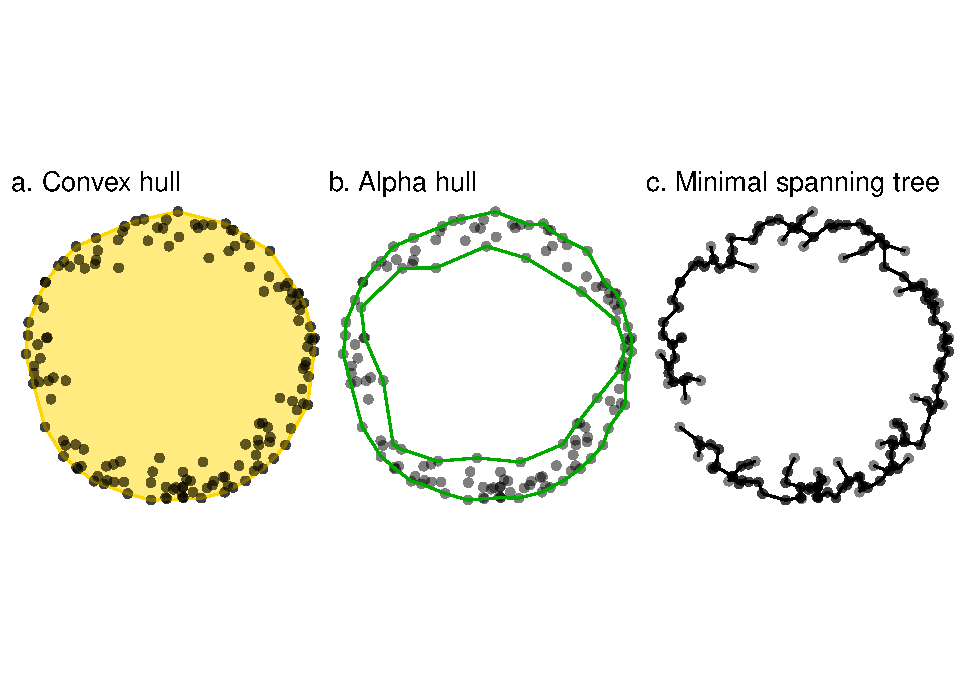
\includegraphics[width=1\linewidth]{mason-lee-laa-cook_files/figure-latex/building-blocks2-1} \caption[The building blocks for graph-based scagnostics]{The building blocks for graph-based scagnostics}(\#fig:building-blocks2)
\end{figure}
\end{Schunk}

\hypertarget{graph-based-scagnostics}{%
\subsection{Graph-based scagnostics}\label{graph-based-scagnostics}}

The nine scagnostics defined in \emph{Scagnostic Distributions} are
detailed below with an explanation, formula, and visualisation. We will
let \emph{A}= alpha Hull \emph{C}= convex hull, \emph{M} = minimum
spanning tree, and \emph{s}= the scagnostic measure. Since some of the
measures have some sample size dependence, we will let \emph{w} be a
constant that adjusts for that.

\begin{itemize}
\tightlist
\item
  \textbf{Convex:} Measure of how convex the shape of the data is.
  Computed as the ratio between the area of the alpha hull (A) and
  convex hull (C).
\end{itemize}

\[s_{convex}=w\frac{area(A)}{area(C)}\]

\begin{Schunk}
\begin{figure}

\includegraphics[width=1\linewidth,height=0.2\textheight]{figures/drawconvex} \caption[Convex Scagnostic Visual Explanation]{Convex Scagnostic Visual Explanation}(\#fig:convexscag)
\end{figure}
\end{Schunk}

\begin{itemize}
\tightlist
\item
  \textbf{Skinny:} A measure of how ``thin'' the shape of the data is.
  It is calculated as the ratio between the area and perimeter of the
  alpha hull (A) with some normalisation such that 0 correspond to a
  perfect circle and values close to 1 indicate a skinny polygon.
\end{itemize}

\[s_{skinny}= 1-\frac{\sqrt{4\pi area(A)}}{perimeter(A)}\]

\begin{Schunk}
\begin{figure}

\includegraphics[width=1\linewidth,height=0.2\textheight]{figures/drawskinny} \caption[Skinny Scagnostic Visual Explanation]{Skinny Scagnostic Visual Explanation}(\#fig:skinnyscag)
\end{figure}
\end{Schunk}

\begin{itemize}
\tightlist
\item
  \textbf{Outlying:} A measure of proportion and severity of outliers in
  dataset. Calculated by comparing the edge lengths of the outlying
  points in the MST with the length of the entire MST.
\end{itemize}

\[s_{outlying}=\frac{length(M_{outliers})}{length(M)}\]

\begin{Schunk}
\begin{figure}

\includegraphics[width=1\linewidth,height=0.2\textheight]{figures/drawoutlying} \caption[Outlying Scagnostic Visual Explanation]{Outlying Scagnostic Visual Explanation}(\#fig:outlyingscag)
\end{figure}
\end{Schunk}

\begin{itemize}
\tightlist
\item
  \textbf{Stringy:} This measure identifies a ``stringy'' shape with no
  branches, such as a thin line of data. It is calculated by comparing
  the number of vertices of degree two (\(V^{(2)}\)) with the total
  number of vertices (\(V\)), dropping those of degree one
  (\(V^{(1)}\)).
\end{itemize}

\[s_{stringy} = \frac{|V^{(2)}|}{|V|-|V^{(1)}|}\]

\begin{Schunk}
\begin{figure}
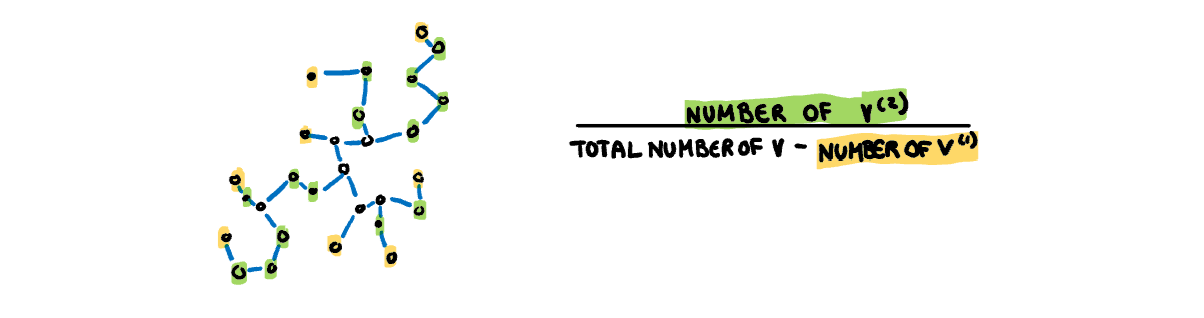
\includegraphics[width=1\linewidth,height=0.2\textheight]{figures/drawstringy} \caption[Stringy Scagnostic Visual Explanation]{Stringy Scagnostic Visual Explanation}(\#fig:stringyscag)
\end{figure}
\end{Schunk}

\begin{itemize}
\tightlist
\item
  \textbf{Skewed:} A measure of skewness in the edge lengths of the MST
  (not in the distribution of the data). It is calculated as the ratio
  between the 40\% IQR and the 80\% IQR, adjusted for sample size
  dependence.
\end{itemize}

\[s_{skewed} = 1-w(1-\frac{q_{90}-{q_{50}}}{q_{90}-q_{10}})\]

\begin{Schunk}
\begin{figure}
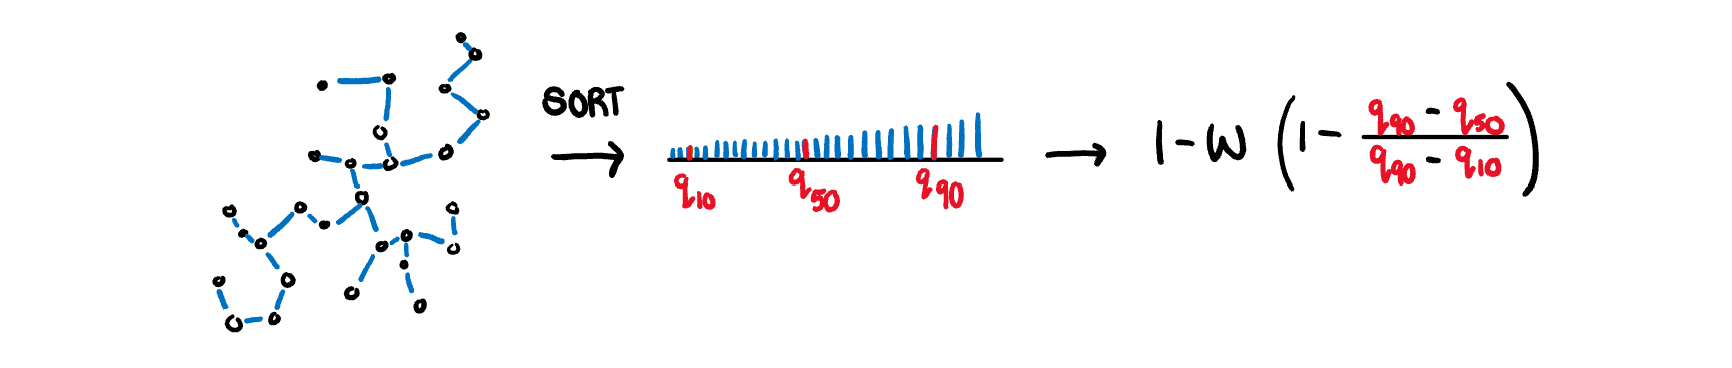
\includegraphics[width=1\linewidth,height=0.2\textheight]{figures/drawskewed} \caption[Skewed Scagnostic Visual Explanation]{Skewed Scagnostic Visual Explanation}(\#fig:skewedscag)
\end{figure}
\end{Schunk}

\begin{itemize}
\tightlist
\item
  \textbf{Sparse:} Identifies if the data is sporadically located on the
  plane. Calculated as the 90th percentile of MST edge lengths.
\end{itemize}

\[s_{sparse}= wq_{90}\]

\begin{Schunk}
\begin{figure}
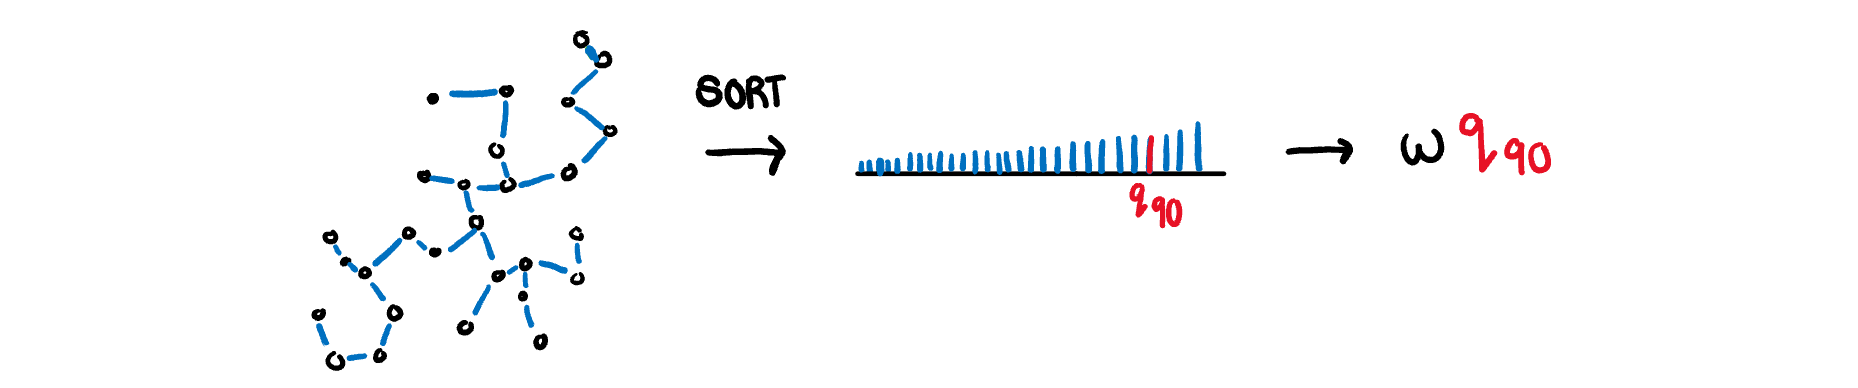
\includegraphics[width=1\linewidth,height=0.2\textheight]{figures/drawsparse} \caption[Sparse Scagnostic Visual Explanation]{Sparse Scagnostic Visual Explanation}(\#fig:sparsescag)
\end{figure}
\end{Schunk}

\begin{itemize}
\tightlist
\item
  \textbf{Clumpy:} This measure is used to detect clustering and is
  calculated through an iterative process. First an edge J is selected
  and removed from the MST. From the two spanning trees that are created
  by this break, we select the largest edge from the smaller tree (K).
  The length of this edge (K) is compared to the removed edge (J) giving
  a clumpy measure for this edge. This process is repeated for every
  edge in the MST and the final clumpy measure is the maximum of this
  value over all edges.
\end{itemize}

\[\max_{j}[1-\frac{\max_{k}[length(e_k)]}{length(e_j)}]\]

\begin{Schunk}
\begin{figure}
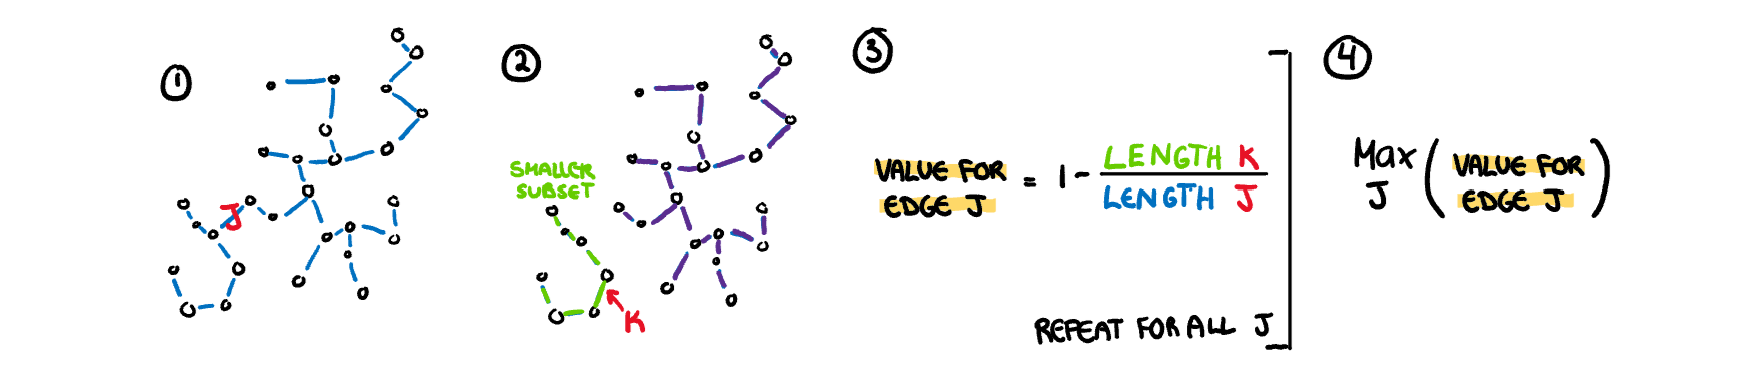
\includegraphics[width=1\linewidth,height=0.2\textheight]{figures/drawclumpy} \caption[Clumpy Scagnostic Visual Explanation]{Clumpy Scagnostic Visual Explanation}(\#fig:clumpyscag)
\end{figure}
\end{Schunk}

\begin{itemize}
\tightlist
\item
  \textbf{Striated:} This measure identifies features such as
  discreteness by finding parallel lines, or smooth algebraic functions.
  Calculated by counting the proportion of acute (0 to 40 degree) angles
  between the adjacent edges of vertices with only two edges.
\end{itemize}

\[\frac1{|V|}\sum_{v \in V^{2}}I(cos\theta_{e(v,a)e(v,b)}<-0.75)\]

\begin{Schunk}
\begin{figure}
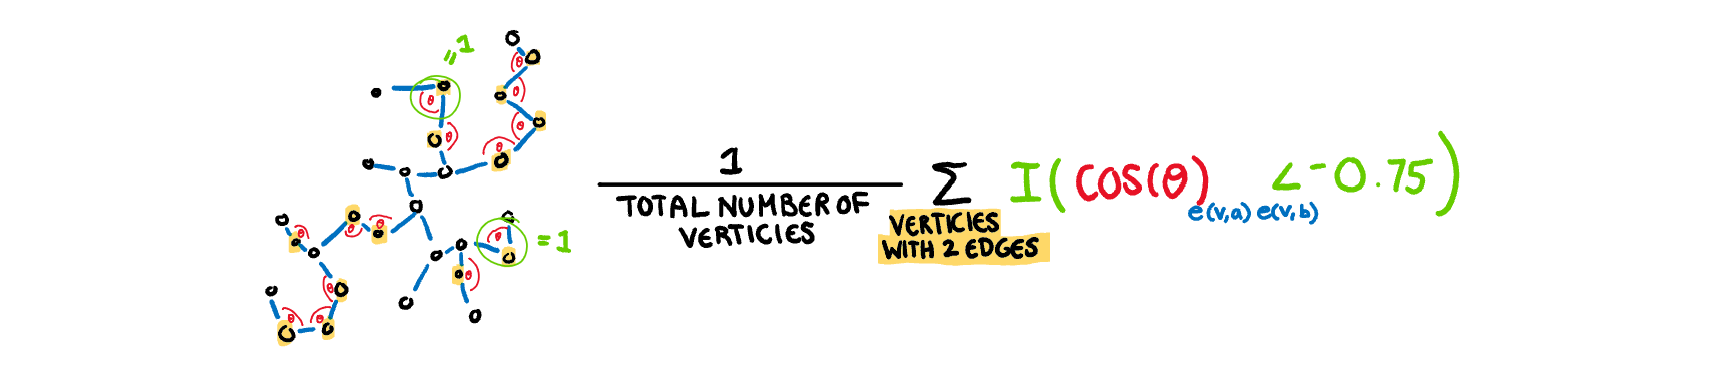
\includegraphics[width=1\linewidth,height=0.2\textheight]{figures/drawstriated} \caption[Striated Scagnostic Visual Explanation]{Striated Scagnostic Visual Explanation}(\#fig:striatedscag)
\end{figure}
\end{Schunk}

\hypertarget{association-based-scagnostics}{%
\subsection{Association-based
scagnostics}\label{association-based-scagnostics}}

\begin{itemize}
\tightlist
\item
  \textbf{Monotonic:} Checks if the data has an increasing or decreasing
  trend. Calculated as the Spearman correlation coefficient, i.e.~the
  Pearson correlation between the ranks of x and y.
\end{itemize}

\[s_{monotonic} = r^2_{spearman}\]

\begin{Schunk}
\begin{figure}
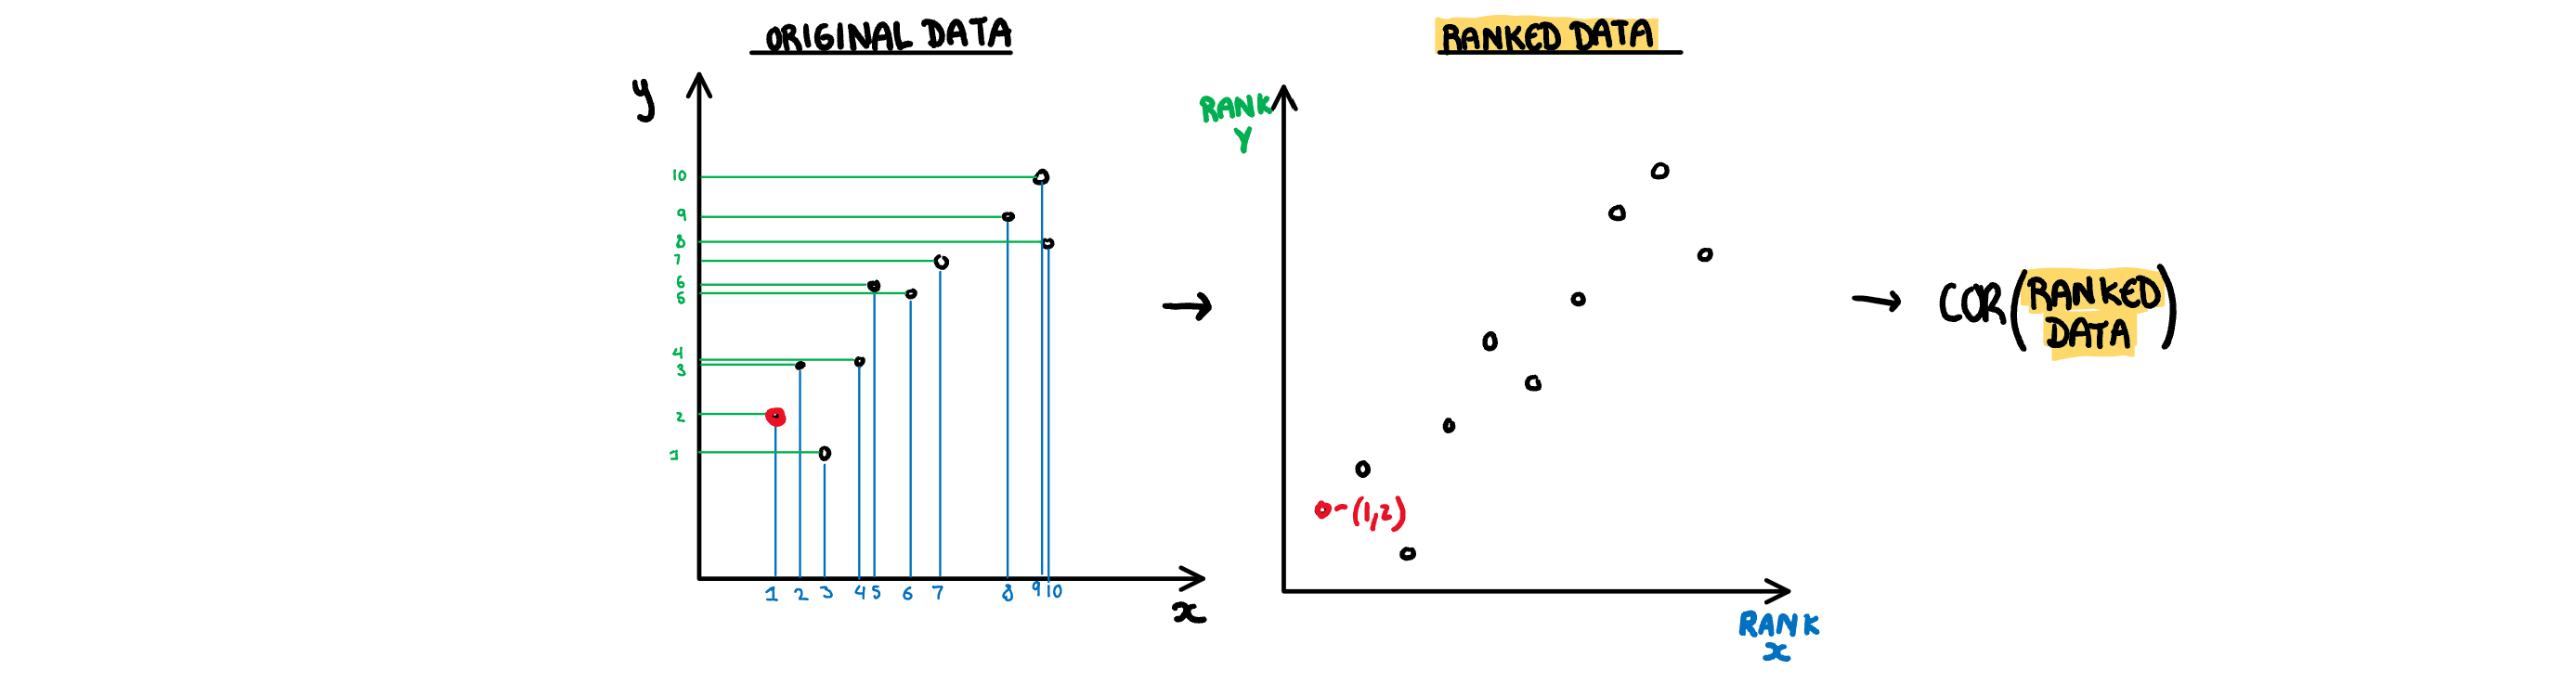
\includegraphics[width=1\linewidth,height=0.2\textheight]{figures/drawmonotonic} \caption[Monotonic Scagnostic Visual Explanation]{Monotonic Scagnostic Visual Explanation}(\#fig:monotonicscag)
\end{figure}
\end{Schunk}

The two additional scagnostics discussed by Katrin Grimm are described
below.

\begin{itemize}
\tightlist
\item
  \textbf{Splines:} Measures the functional non-linear dependence by
  fitting a penalised splines model on X using Y, and on Y using X. The
  variance of the residuals are scaled down by the axis so they are
  comparable, and finally the maximum is taken. Therefore the value will
  be closer to 1 if either relationship can be decently explained by a
  splines model.
\end{itemize}

\[s_{splines}=\max_{i\in x,y}[1-\frac{Var(Residuals_{model~i=.})}{Var(i)}]\]

\begin{Schunk}
\begin{figure}
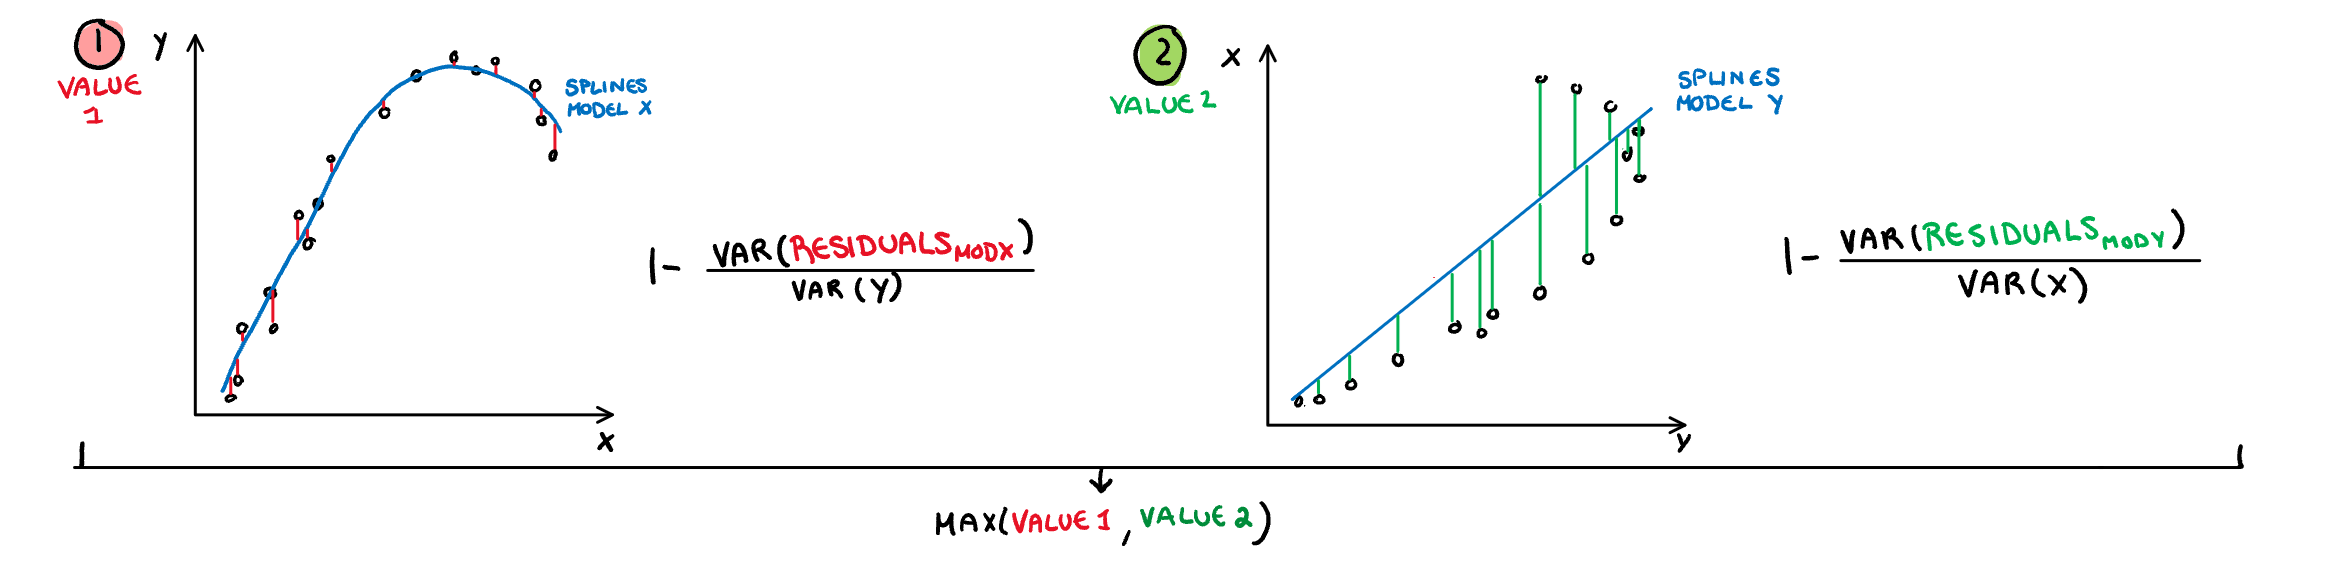
\includegraphics[width=1\linewidth,height=0.2\textheight]{figures/drawsplines} \caption[Splines Scagnostic Visual Explanation]{Splines Scagnostic Visual Explanation}(\#fig:splinescag)
\end{figure}
\end{Schunk}

\begin{itemize}
\tightlist
\item
  \textbf{Dcor:} A measure of non-linear dependence which is 0 if and
  only if the two variables are independent. Computed using an ANOVA
  like calculation on the pairwise distances between observations.
\end{itemize}

\[s_{dcor}= \sqrt{\frac{\mathcal{V}(X,Y)}{\mathcal{V}(X,X)\mathcal{V}(Y,Y)}}\]\\
where \[\mathcal{V}
(X,Y)=\frac{1}{n^2}\sum_{k=1}^n\sum_{l=1}^nA_{kl}B_{kl}\]\\
where \[A_{kl}=a_{kl}-\bar{a}_{k.}-\bar{a}_{.j}-\bar{a}_{..}\]
\[B_{kl}=b_{kl}-\bar{b}_{k.}-\bar{b}_{.j}-\bar{b}_{..}\]

\begin{Schunk}
\begin{figure}
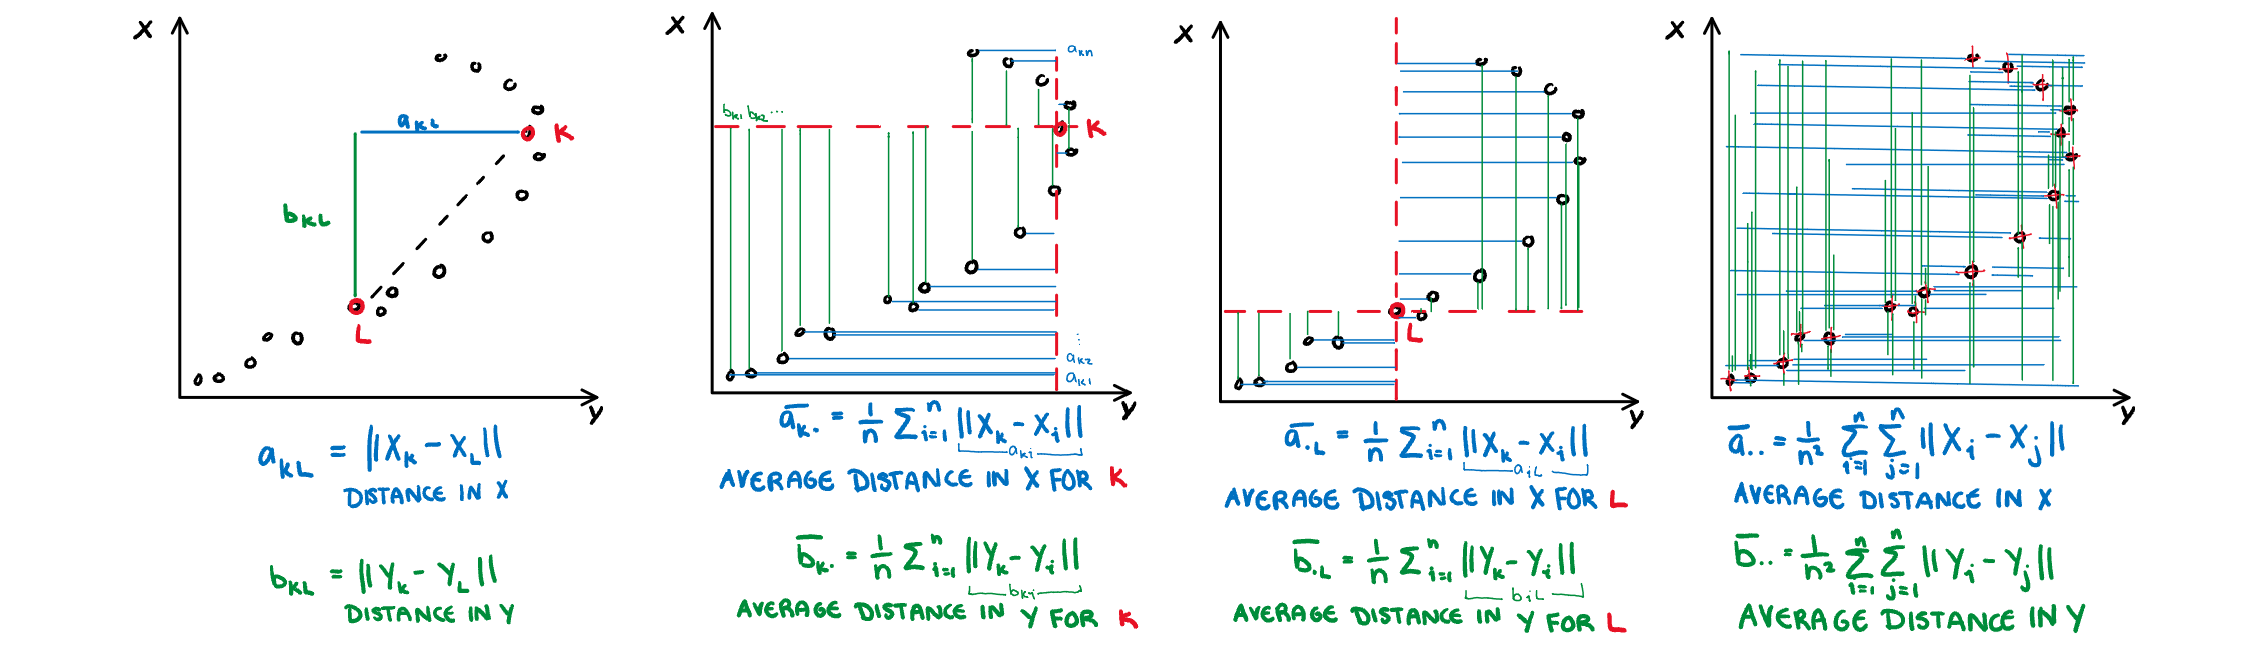
\includegraphics[width=1\linewidth,height=0.2\textheight]{figures/drawdcor} \caption[Dcor Scagnostic Visual Explanation]{Dcor Scagnostic Visual Explanation}(\#fig:dcorscag)
\end{figure}
\end{Schunk}

\hypertarget{checking-the-scagnostics-calculations}{%
\subsection{Checking the scagnostics
calculations}\label{checking-the-scagnostics-calculations}}

Once we have working functions that correctly calculate the scagnostics
according to their definition, we can assess how well they identify the
visual features of scatter plots. To test the packages ability to
differentiate plots, we have creates a dataset called ``features'' (that
is also in the Cassowaryr package) that contains a series of interesting
and unique scatter plots which we can run our scagnsotics on.

\begin{Schunk}
\begin{figure}
\includegraphics[width=1\linewidth]{mason-lee-laa-cook_files/figure-latex/Features plot-1} \caption[The Scatter Plots of the Features Dataset]{The Scatter Plots of the Features Dataset}(\#fig:Features plot)
\end{figure}
\end{Schunk}

These scatter plots typify certain visual features we want to look for
in scatter plots, be it deterministic relationships (such as that shown
in the nonlinear feature), discreteness in variables (vlines), or
clustering (clumpy), we should be able to use scagnostics to identify
each of these scatter plots. Below is a visual table of an example of a
high, a moderate, and a low value, on each scagnostic. The scagnostics
are supposed to range from 0 to 1 however in some cases the values are
so compressed that a moderate value would not fit, indicating that the
scagnostics do not work quite as intended. We suspect the reason for
these warped distributions is the removal of binning as a preliminary
step in calculating the scagnostics. We wanted the package to have
binning as an optional method, considering choices in binning can lead
to bias as noted in ``Scagnostic Distributions'' \citep{scagdist} or
unreproducible results as noted in ``Robustness of Scagnostics'' .
Therefore the current scagnostics will be assessed without binning
\citep{robust}.

\begin{Schunk}
\begin{figure}
\includegraphics[width=1\linewidth]{mason-lee-laa-cook_files/figure-latex/Visual Table-1} \caption[The Features Scatterplots in a Visual Table]{The Features Scatterplots in a Visual Table}(\#fig:Visual Table)
\end{figure}
\end{Schunk}

This plot gives a slight idea of the issues some of the scagnsotics face
in their current state. The scagnostics based upon the convex hull
(i.e.~skinny and convex) work fine, as do the association measures such
as montonic, dcor and splines. The main issue comes from the measures
based on the MST, and their issues largely come from binning. The MST
measures and their issues are:

\begin{itemize}
\item
  \textbf{Striated}: striated can identify the specific case of one
  discrete variable and one continuous variable (which alone is not
  particularly interesting) but will not identify two discrete
  variables. Since by definition it is a subset of the stringy measure,
  they are highly correlated, which means most variables that score
  highly on striated already score highly on stringy, making the measure
  less useful.
\item
  \textbf{Sparse}: While sparse does seem to identify spread out
  distributions, it rarely returns a value higher than 0.1. As this
  measure is the 90th percentile of MST edge lengths, and the removal of
  binning allows for a large number of arbitrarily small edges. In
  addiiton to this, a larger number of observations will arbitrarily
  make this value smaller. The addition of new points will increase the
  number of small edges and decrease the number of large edges, and it
  is rare that a significantly large edge will be at or below the 90th
  percentile.
\item
  \textbf{Skewed}: this measure can identify skewed edge lengths (such
  as the L shape in the visual table) however the values on real data
  rarely drop below 0.5 or rise above 0.8. Skewed seems to suffers from
  the same issue as sparse reguarding the binning issue and is also
  heavily influenced by the number of observations in the scatter plot.
\item
  \textbf{Outlying}: the disctinction of outlying points described in
  the scagnostic literature is certainly strange. By definition an
  outlier must have \emph{all} its adjacent edges in the MST above this
  threshold, and the visual table displays three interesting cases of
  this. The first plot (outliers2) returns a 0 even though the handful
  of points in the top corner would likely be considered to be outliers
  by a human. This is because within that group the points are close
  enough that all of them have at least one edge that is below the
  outlying threshold. Even if we changed the measure such that only one
  edge needed to be above the outlying threshold, it would only remove a
  single point. The l-shape shows an increasing spread of the points as
  they move away from the bottom left corner, as such, the larger edge
  lengths make sense within the distribution. Outlying does not take
  this into account, and identifies a large number of the spread out
  points to be outliers and removes them before computing the other
  scagnsotics. The value that scores the highest on the outlying measure
  is, without question, a highly outlying distribution, however the
  outlying measure only returns a 0.5, this is again due to the removal
  of binning as a preprocessing step.
\item
  \textbf{Clumpy}: the clumpy scagnostic is probably the one that
  suffers the most with the removal of the binning step. Due to it being
  a ratio between an edge and its longest adjacent edge, it does not
  identify the largest edge, but rather an edge that is connected to an
  arbitrarily small edge. Because of this, this scagnsotic reliably
  returns an arbitrarily high value and scatter plots that actually
  contains clusters (such as clusters) scores low on this measure, while
  a continuous variable plotted against a discrete variable score
  arbitrarily high.
\item
  \textbf{Stringy}: This measure rarely drops below 0.5 even on data
  generated from a random normal distribution (which should intuitively
  return a 0). Unlike the other scagnostics on this list, stringy does
  not depend upon the edge lengths of the MST, so it is hard to say if
  this issue stems from binning.
\end{itemize}

With these issues in mind, we have defines and written several new
scagnostics that work even without the pre-processing seto of binning.

\hypertarget{the-adjusted-scagnostics-measures}{%
\subsubsection{The Adjusted Scagnostics
Measures}\label{the-adjusted-scagnostics-measures}}

The measures that need an adjusted version are striated, sparse, skewed,
and clumpy. The outlying and stringy measure could possibly be left as
they are, as they are not as badly damaged by the removal of binning.

\hypertarget{striated-adjusted}{%
\paragraph{Striated Adjusted}\label{striated-adjusted}}

The issues surrounding the striated scagnostic are:

\begin{enumerate}
\def\labelenumi{\arabic{enumi}.}
\item
  By only counting vertices with 2 edges, the set of vertices counted in
  this measure are a subset of those counted in stringy, thus the two
  meaures are highly correlated.
\item
  In order for the vertex to be counted, the angle between the edges
  needs to be approximately 135 to 220 degrees. The original idea seems
  to have been to identify the predominantly 180 degree angles that come
  with a discrete variable plotted against a continuous one, however the
  large margin of error just makes the measure almost identical to
  stringy.
\end{enumerate}

To account for these two issues the striated adjusted measure considers
all vertices (not just those with two adjacent edges), and makes the
measure strict around the 180 and 90 degree angles. With this we can see
the improvements on the measure.

\begin{Schunk}
\begin{figure}
\includegraphics[width=1\linewidth]{mason-lee-laa-cook_files/figure-latex/Striated Vtable-1} \caption[A Visual Table Comparison of Striated and Striated 2]{A Visual Table Comparison of Striated and Striated 2}(\#fig:Striated Vtable)
\end{figure}
\end{Schunk}

While these two measures may seem similar at a glace, there are a few
minor things that make the striated2 scagnsotic an improvement on the
stirated scagnsotic. First of all, the perfect 1 value on striated goes
to the ``line'' scatter plot. While this does fulfil the definition, it
is not what the measure is supposed to be looking for, rather supposed
to be identifying the ``vlines'' scatter plot. Since striated does not
count the right angles that go between the vertical lines, a truely
striated plot will never get a full 1 on this measure, striated adjusted
fixes this. After that there is a large gap in both measures because
none of the other scatter plots have a strictly discrete measure on the
x or y axis. The lower plots show that striated2 is also better at
identifying discrete relationships with a rotation and noise added as
shown in the ``discrete'' plot. In striated ``discrete'' is lower in the
order than ``outlying'' which would indicate that striated has finished
looking at discreteness. In striated2, after the plots with strict
discreteness in ``vlines'' or strict rotated disceteness in ``line'', is
the noisey and rotated ``discrete'' plot. Therefore in terms of ordering
the plots in how well they represent the feature of discreteness,
striated2 outperforms striated.

The scagnsotics need to be used and interpreted with the type of dataset
you are working with in mind. For if we are looking at a dataset that is
discrete, a very low value on striated2 would indicate some strange
relationship in the scatter plot. Since the old striated measure is
specifically trying to find a continuous variable against a discrete
variable, its highest values are also identified by the striated2. The
lowest values on striated simply identify a plot where all the variables
are at right angles, once again a measure of disceteness but one that is
not identified by striated. Striated2 encapsulates both versions of
discreteness in the values that get exactly a 1.

\hypertarget{clumpy-adjusted}{%
\paragraph{Clumpy Adjusted}\label{clumpy-adjusted}}

The issues that need to be addressed with the new clumpy measure are:

\begin{enumerate}
\def\labelenumi{\arabic{enumi}.}
\item
  It needs to consider more than 1 edge in its final measure to make the
  measure more robust
\item
  The impact of the ratio between the long and short edges need to be
  weighted by the size of their clusters so the measure does not simply
  identify outliers
\item
  It should not consider vertices that's adjacent angles form a straight
  line (to avoid identifying the angles striated identifies)
\end{enumerate}

Before we calculated a new clumpy measure, we looked into applying a
different adjustment defined in the \emph{Improving the robustness of
scagnsotics} that is a robust version of the original clumpy measure
\citep{robust}. This version of clumpy has been included in the package
as ``clumpy\_r'' however it is not included as an option in the higher
level functions such as calc\_scags() because its computation time is
too long. This measure tries to build multiple clusters, each having
their own clumpy value, and then returns the weighted sum, where each
value is weighted by the number of observations in that cluster. This
version of clumpy spreads the scatter plots more evenly between 0 and 1
and is more robust to outliers, however it does a poor job of ordering
plots generally considered to be clumpy without the assistance of
binning. Since this scagnostic cannot be used in large scale scagnostic
calculations (such as those done on every pairwise combination of
variables as is intended by the package) and it maintains the ordering
issue from the original measure, it is not discussed here.

Therefore in order to fix the issues in the clumpy measure described
above, we designed an adjusted clumpy measure, called clumpy2 in the
package, and it is calculated as follows:

\begin{enumerate}
\def\labelenumi{\arabic{enumi}.}
\tightlist
\item
  Sort the edges in the MST
\item
  Calculate the difference of adjacent vectors in this ordering, and
  find the index of the maximum. This maximum difference should indicate
  the jump from between cluster edges and inter-cluster edges.
\item
  Remove the between cluster edges from the MST and build clusters using
  the remaining edges
\item
  For each between cluster edge, take the smaller cluster (in number of
  observations) and take its median edge length. The clumpy value for
  that edge is the ratio between the large and small edge lengths
  \(\frac{edge_{small}}{edge_{large}}\), with a two multiplicative
  penaltys, one for uneven clusters
  \(\frac{2\times n_{small}}{n_{small}+n_{big}}\), and one for
  ``stringy'' scatter plots that is only applied if the stringy value is
  higher than 0.95, to reduce the arbitrarily large clumpy scores that
  come from striated plots \(1-s_{stringy}\).
\item
  Take the mean clumpy value for each between cluster edge, if it is
  below 1 it is beneath the threshold that is consdiered clumpy, and the
  value is adjusted to 1.
\item
  Clumpy 2 returns \(1-\frac{1}{mean(clumpy_i)}\)
\end{enumerate}

With this calculation, we generate the clumpy2 measure which is compared
to the original clumpy measure in the figure below.

\begin{Schunk}
\begin{figure}
\includegraphics[width=1\linewidth]{mason-lee-laa-cook_files/figure-latex/Clumpy Vtable-1} \caption[A Visual Table Comparison of Clumpy and Clumpy 2]{A Visual Table Comparison of Clumpy and Clumpy 2}(\#fig:Clumpy Vtable)
\end{figure}
\end{Schunk}

Here we can see the improvements made on the clumpy measure in both
distribution from 0 to 1 and ordering. The measure is more spread out,
and so values range more accurately from 0 to 1. More importantly the
measures do a better job of ordering the scatter plots. On the original
clumpy measure the ``clusters'' scatter plot was next to last, on the
clumpy2 measure ``clusters'' is is identified as the most clumpy scatter
plot. Clumpy 2 also has a penalty for uneven clusters (to avoid being
large due to a small colelction of outliers) and clusters created
arbitrarily due to discreteness (such as vlines) in order to better
aling with the human interpretation of clumpy. With these changes, the
stronger performance of clumpy2 is apparent in this visual table.

\hypertarget{implementation}{%
\section{Implementation}\label{implementation}}

\hypertarget{installation}{%
\subsection{Installation}\label{installation}}

The package can be installed using

\begin{verbatim}
install.packages("cassowaryr")
\end{verbatim}

from CRAN and using

\begin{verbatim}
remotes::install_github("numbats/cassowaryr")
\end{verbatim}

installs the development version.

\hypertarget{web-site}{%
\subsection{Web site}\label{web-site}}

More documentation of the package can be found at the web site
\url{https://numbats.github.io/cassowaryr/}.

\hypertarget{data-sets}{%
\subsection{Data sets}\label{data-sets}}

The cassowaryr package comes with several data sets that load with the
package, they are described here.

\begin{Schunk}

\begin{tabular}{l|l}
\hline
dt & text\\
\hline
features & Simulated data with special features.\\
\hline
anscombe\_tidy & Data from Anscombes famous example in tidy format.\\
\hline
datasaurus\_dozen & Datasaurus Dozen data in a long tidy format.\\
\hline
datasaurus\_dozen\_wide & Datasaurus Dozen Data in a wide tidy format.\\
\hline
numbat & A toy data set with a numbat shape hidden among noise variables.\\
\hline
pk & Parkinsons data from UCI machine learning archive.\\
\hline
\end{tabular}

\end{Schunk}

\hypertarget{functions}{%
\subsection{Functions}\label{functions}}

\hypertarget{scagnostics-functions}{%
\subsubsection{Scagnostics functions}\label{scagnostics-functions}}

The scagnostics functions functions either calculate each scagnostic
measure, or are involved in the process of calcuating a scanostic
measure (such as making the hull objects). These functions are low level
functions, and while they are exported and can be used, they are not the
intended method of calcuating scagnostics as they perform no outlier
removal, however they are still an option for users if they wish. In
some cases, such as sc\_clumpy\_r for clumpy robust, they are the only
method to calculate that scagnostic. the The functions in this group
are:

\begin{Schunk}

\begin{tabular}{l|l}
\hline
dt & text\\
\hline
scree & Generates a scree object that contains the Delaunay triangulation of the scater plot.\\
\hline
sc\_clumpy & Compute the original clumpy scagnostic measure.\\
\hline
sc\_clumpy2 & Compute adjusted clumpy scagnositc measure.\\
\hline
sc\_clumpy\_r & Compute robust clumpy scagnostic measure.\\
\hline
sc\_convex & Compute the original convex scagnostic measure\\
\hline
sc\_dcor & Compute the distance correlation index.\\
\hline
sc\_monotonic & Compute the Spearman correlation.\\
\hline
sc\_outlying & Compute the original outlying scagnostic measure.\\
\hline
sc\_skewed & Compute the original skewed scagnostic measure.\\
\hline
sc\_skinny & Compute the original skinny scagnostic measure.\\
\hline
sc\_sparse & Compute the original sparse scagnostic measure.\\
\hline
sc\_sparse2 & Compute adjusted sparse measure.\\
\hline
sc\_splines & Compute the spline based index.\\
\hline
sc\_striated & Compute the original stirated scagnostic measure.\\
\hline
sc\_striated2 & Compute angle adjusted striated measure.\\
\hline
sc\_stringy & Compute stringy scagnostic measure.\\
\hline
\end{tabular}

\end{Schunk}

\hypertarget{drawing-functions}{%
\subsubsection{Drawing functions}\label{drawing-functions}}

The drawing functions are intended to be used my the user so they can
better understand the results of the scagnostic functions. The input is
two numeric vectors and the output is a ggplot object that draws the
graph based object in question. The functions that belong to this group
are:

\begin{Schunk}

\begin{tabular}{l|l}
\hline
func\_name & description\\
\hline
draw\_alphahull & Drawing the alpha hull.\\
\hline
draw\_convexhull & Drawing the convex hull.\\
\hline
draw\_mst & Drawing the MST.\\
\hline
\end{tabular}

\end{Schunk}

\hypertarget{summary-functions}{%
\subsubsection{Summary functions}\label{summary-functions}}

The summary functions are the perferred method for users to calculate
scagnostics. The calc\_scags function is supposed to be used on long
data with the dplyr group\_by and summarise functions. the
calc\_scags\_wide functions is designed to take in a tibble of numerical
variables and return the scagnostics on every possible pairwise scatter
plot. Both functions return a tibble where each column is a scagnostics.
These are the two main functions of the package. The main arguments of
the calc\_scags function are shown in **Table \_\_**.

\begin{Schunk}

\begin{tabular}{l|l}
\hline
func\_name & description\\
\hline
calc\_scags & Compute selected scagnostics on subsets.\\
\hline
calc\_scags\_widet & Compute scagnostics on all possible scatter plots for the given data.\\
\hline
\end{tabular}

\end{Schunk}

\begin{Schunk}

\begin{tabular}{l|l}
\hline
argument & description\\
\hline
y & numeric vector of x values.\\
\hline
x & numeric vector of y values.\\
\hline
scags & collection of strings matching names of scagnostics to calculate: outlying, stringy, striated, striated2, striped, clumpy, clumpy2, sparse, skewed, convex, skinny, monotonic, splines, dcor. The default is to calculate all scagnostics.\\
\hline
\end{tabular}

\end{Schunk}

While the calc\_scags function does not take in a tibble, it is designed
to be seamlessly integrated into the tidy\_data format, for example,
using the code below, we can calculate a specified list of scagnostics
on the scatter plots from the features data, producing the output shown
in **Table \_\_**.

\begin{Schunk}
\begin{Sinput}
features_scags <- features %>%
  group_by(feature) %>%
  summarise(calc_scags(x,y), scags=c("outlying", "clumpy2", "splines"))
\end{Sinput}
\end{Schunk}

\begin{Schunk}

\begin{tabular}{l|r|r|r|r|r|r|r|r|r|r|r|r|r|l}
\hline
feature & outlying & stringy & striated & striated2 & clumpy & clumpy2 & sparse & skewed & convex & skinny & monotonic & splines & dcor & scags\\
\hline
barrier & 0.0000000 & 0.7560976 & 0.2307692 & 0.0588235 & 0.8104995 & 0.0000000 & 0.0958269 & 0.5244451 & 0.8176685 & 0.2423652 & 0.3480849 & 0.2533140 & 0.3719488 & outlying\\
\hline
barrier & 0.0000000 & 0.7560976 & 0.2307692 & 0.0588235 & 0.8104995 & 0.0000000 & 0.0958269 & 0.5244451 & 0.8176685 & 0.2423652 & 0.3480849 & 0.2533140 & 0.3719488 & clumpy2\\
\hline
barrier & 0.0000000 & 0.7560976 & 0.2307692 & 0.0588235 & 0.8104995 & 0.0000000 & 0.0958269 & 0.5244451 & 0.8176685 & 0.2423652 & 0.3480849 & 0.2533140 & 0.3719488 & splines\\
\hline
clusters & 0.0551486 & 0.7027027 & 0.2721088 & 0.0827586 & 0.8015825 & 0.8349580 & 0.0600144 & 0.5607868 & 0.4872930 & 0.5192027 & 0.0343677 & 0.6079558 & 0.3754130 & outlying\\
\hline
clusters & 0.0551486 & 0.7027027 & 0.2721088 & 0.0827586 & 0.8015825 & 0.8349580 & 0.0600144 & 0.5607868 & 0.4872930 & 0.5192027 & 0.0343677 & 0.6079558 & 0.3754130 & clumpy2\\
\hline
clusters & 0.0551486 & 0.7027027 & 0.2721088 & 0.0827586 & 0.8015825 & 0.8349580 & 0.0600144 & 0.5607868 & 0.4872930 & 0.5192027 & 0.0343677 & 0.6079558 & 0.3754130 & splines\\
\hline
discrete & 0.0000000 & 0.7065217 & 0.2809917 & 0.0756303 & 0.8068468 & 0.0000000 & 0.1077328 & 0.7105037 & 0.9317297 & 0.0714153 & 0.0082035 & 0.0000905 & 0.1043876 & outlying\\
\hline
discrete & 0.0000000 & 0.7065217 & 0.2809917 & 0.0756303 & 0.8068468 & 0.0000000 & 0.1077328 & 0.7105037 & 0.9317297 & 0.0714153 & 0.0082035 & 0.0000905 & 0.1043876 & clumpy2\\
\hline
discrete & 0.0000000 & 0.7065217 & 0.2809917 & 0.0756303 & 0.8068468 & 0.0000000 & 0.1077328 & 0.7105037 & 0.9317297 & 0.0714153 & 0.0082035 & 0.0000905 & 0.1043876 & splines\\
\hline
disk & 0.0185229 & 0.7542373 & 0.3154362 & 0.0408163 & 0.9276877 & 0.4045036 & 0.0820240 & 0.5791372 & 0.8778536 & 0.1431009 & 0.0855451 & 0.0973406 & 0.1792892 & outlying\\
\hline
disk & 0.0185229 & 0.7542373 & 0.3154362 & 0.0408163 & 0.9276877 & 0.4045036 & 0.0820240 & 0.5791372 & 0.8778536 & 0.1431009 & 0.0855451 & 0.0973406 & 0.1792892 & clumpy2\\
\hline
disk & 0.0185229 & 0.7542373 & 0.3154362 & 0.0408163 & 0.9276877 & 0.4045036 & 0.0820240 & 0.5791372 & 0.8778536 & 0.1431009 & 0.0855451 & 0.0973406 & 0.1792892 & splines\\
\hline
gaps & 0.0000000 & 0.7142857 & 0.2868852 & 0.0750000 & 0.9075206 & 0.7520619 & 0.0984819 & 0.5824063 & 0.8171231 & 0.2187712 & 0.0572168 & 0.0417080 & 0.1321236 & outlying\\
\hline
gaps & 0.0000000 & 0.7142857 & 0.2868852 & 0.0750000 & 0.9075206 & 0.7520619 & 0.0984819 & 0.5824063 & 0.8171231 & 0.2187712 & 0.0572168 & 0.0417080 & 0.1321236 & clumpy2\\
\hline
gaps & 0.0000000 & 0.7142857 & 0.2868852 & 0.0750000 & 0.9075206 & 0.7520619 & 0.0984819 & 0.5824063 & 0.8171231 & 0.2187712 & 0.0572168 & 0.0417080 & 0.1321236 & splines\\
\hline
l-shape & 0.3849340 & 0.7534247 & 0.2765957 & 0.0434783 & 0.8783569 & 0.0000000 & 0.0528575 & 0.7884859 & 0.0684984 & 0.7013534 & 0.4797960 & 0.1924127 & 0.4621725 & outlying\\
\hline
l-shape & 0.3849340 & 0.7534247 & 0.2765957 & 0.0434783 & 0.8783569 & 0.0000000 & 0.0528575 & 0.7884859 & 0.0684984 & 0.7013534 & 0.4797960 & 0.1924127 & 0.4621725 & clumpy2\\
\hline
l-shape & 0.3849340 & 0.7534247 & 0.2765957 & 0.0434783 & 0.8783569 & 0.0000000 & 0.0528575 & 0.7884859 & 0.0684984 & 0.7013534 & 0.4797960 & 0.1924127 & 0.4621725 & splines\\
\hline
line & 0.1137124 & 1.0000000 & 0.9863946 & 1.0000000 & 0.9527164 & 0.0000000 & 0.0237047 & 0.7792845 & 0.0000000 & 1.0000000 & 1.0000000 & 1.0000000 & 1.0000000 & outlying\\
\hline
line & 0.1137124 & 1.0000000 & 0.9863946 & 1.0000000 & 0.9527164 & 0.0000000 & 0.0237047 & 0.7792845 & 0.0000000 & 1.0000000 & 1.0000000 & 1.0000000 & 1.0000000 & clumpy2\\
\hline
line & 0.1137124 & 1.0000000 & 0.9863946 & 1.0000000 & 0.9527164 & 0.0000000 & 0.0237047 & 0.7792845 & 0.0000000 & 1.0000000 & 1.0000000 & 1.0000000 & 1.0000000 & splines\\
\hline
nonlinear1 & 0.2715451 & 1.0000000 & 0.9863014 & 1.0000000 & 0.9530983 & 0.0000000 & 0.0259366 & 0.8006017 & 0.7104439 & 0.3267782 & 0.1684822 & 0.9999054 & 0.5956946 & outlying\\
\hline
nonlinear1 & 0.2715451 & 1.0000000 & 0.9863014 & 1.0000000 & 0.9530983 & 0.0000000 & 0.0259366 & 0.8006017 & 0.7104439 & 0.3267782 & 0.1684822 & 0.9999054 & 0.5956946 & clumpy2\\
\hline
nonlinear1 & 0.2715451 & 1.0000000 & 0.9863014 & 1.0000000 & 0.9530983 & 0.0000000 & 0.0259366 & 0.8006017 & 0.7104439 & 0.3267782 & 0.1684822 & 0.9999054 & 0.5956946 & splines\\
\hline
nonlinear2 & 0.0000000 & 0.7435897 & 0.3200000 & 0.0816327 & 0.7417817 & 0.0000000 & 0.0531586 & 0.6008527 & 0.2178211 & 0.6724595 & 0.8094209 & 0.9738497 & 0.8736559 & outlying\\
\hline
nonlinear2 & 0.0000000 & 0.7435897 & 0.3200000 & 0.0816327 & 0.7417817 & 0.0000000 & 0.0531586 & 0.6008527 & 0.2178211 & 0.6724595 & 0.8094209 & 0.9738497 & 0.8736559 & clumpy2\\
\hline
nonlinear2 & 0.0000000 & 0.7435897 & 0.3200000 & 0.0816327 & 0.7417817 & 0.0000000 & 0.0531586 & 0.6008527 & 0.2178211 & 0.6724595 & 0.8094209 & 0.9738497 & 0.8736559 & splines\\
\hline
outliers & 0.0000000 & 0.6923077 & 0.2761905 & 0.0970874 & 0.8656430 & 0.5248417 & 0.0749958 & 0.5730171 & 0.4265678 & 0.4658078 & 0.7051628 & 0.6247843 & 0.7329544 & outlying\\
\hline
outliers & 0.0000000 & 0.6923077 & 0.2761905 & 0.0970874 & 0.8656430 & 0.5248417 & 0.0749958 & 0.5730171 & 0.4265678 & 0.4658078 & 0.7051628 & 0.6247843 & 0.7329544 & clumpy2\\
\hline
outliers & 0.0000000 & 0.6923077 & 0.2761905 & 0.0970874 & 0.8656430 & 0.5248417 & 0.0749958 & 0.5730171 & 0.4265678 & 0.4658078 & 0.7051628 & 0.6247843 & 0.7329544 & splines\\
\hline
outliers2 & 0.5906739 & 0.7378641 & 0.2556391 & 0.0916031 & 0.8168932 & 0.0000000 & 0.0752187 & 0.5544897 & 0.6363848 & 0.2571140 & 0.0600126 & 0.1437244 & 0.2247284 & outlying\\
\hline
outliers2 & 0.5906739 & 0.7378641 & 0.2556391 & 0.0916031 & 0.8168932 & 0.0000000 & 0.0752187 & 0.5544897 & 0.6363848 & 0.2571140 & 0.0600126 & 0.1437244 & 0.2247284 & clumpy2\\
\hline
outliers2 & 0.5906739 & 0.7378641 & 0.2556391 & 0.0916031 & 0.8168932 & 0.0000000 & 0.0752187 & 0.5544897 & 0.6363848 & 0.2571140 & 0.0600126 & 0.1437244 & 0.2247284 & splines\\
\hline
positive & 0.1380011 & 0.7600000 & 0.2315789 & 0.0537634 & 0.8064850 & 0.2864513 & 0.0698193 & 0.5492786 & 0.7065185 & 0.4383215 & 0.9206001 & 0.8511705 & 0.9120633 & outlying\\
\hline
positive & 0.1380011 & 0.7600000 & 0.2315789 & 0.0537634 & 0.8064850 & 0.2864513 & 0.0698193 & 0.5492786 & 0.7065185 & 0.4383215 & 0.9206001 & 0.8511705 & 0.9120633 & clumpy2\\
\hline
positive & 0.1380011 & 0.7600000 & 0.2315789 & 0.0537634 & 0.8064850 & 0.2864513 & 0.0698193 & 0.5492786 & 0.7065185 & 0.4383215 & 0.9206001 & 0.8511705 & 0.9120633 & splines\\
\hline
ring & 0.0189650 & 0.7627119 & 0.3087248 & 0.0816327 & 0.9389213 & 0.4493065 & 0.0652138 & 0.6540108 & 0.2572840 & 0.7189457 & 0.0446935 & 0.0035393 & 0.2341579 & outlying\\
\hline
ring & 0.0189650 & 0.7627119 & 0.3087248 & 0.0816327 & 0.9389213 & 0.4493065 & 0.0652138 & 0.6540108 & 0.2572840 & 0.7189457 & 0.0446935 & 0.0035393 & 0.2341579 & clumpy2\\
\hline
ring & 0.0189650 & 0.7627119 & 0.3087248 & 0.0816327 & 0.9389213 & 0.4493065 & 0.0652138 & 0.6540108 & 0.2572840 & 0.7189457 & 0.0446935 & 0.0035393 & 0.2341579 & splines\\
\hline
vlines & 0.0000000 & 0.9722222 & 0.9333333 & 1.0000000 & 0.9890221 & 0.1708173 & 0.0479482 & 0.7603892 & 0.9584572 & 0.1308428 & 0.0824344 & 0.0000000 & 0.1039919 & outlying\\
\hline
vlines & 0.0000000 & 0.9722222 & 0.9333333 & 1.0000000 & 0.9890221 & 0.1708173 & 0.0479482 & 0.7603892 & 0.9584572 & 0.1308428 & 0.0824344 & 0.0000000 & 0.1039919 & clumpy2\\
\hline
vlines & 0.0000000 & 0.9722222 & 0.9333333 & 1.0000000 & 0.9890221 & 0.1708173 & 0.0479482 & 0.7603892 & 0.9584572 & 0.1308428 & 0.0824344 & 0.0000000 & 0.1039919 & splines\\
\hline
weak & 0.0491130 & 0.7532468 & 0.2244898 & 0.0520833 & 0.7601166 & 0.0000000 & 0.1139095 & 0.6607944 & 0.8445384 & 0.1878559 & 0.4080648 & 0.1699943 & 0.3973523 & outlying\\
\hline
weak & 0.0491130 & 0.7532468 & 0.2244898 & 0.0520833 & 0.7601166 & 0.0000000 & 0.1139095 & 0.6607944 & 0.8445384 & 0.1878559 & 0.4080648 & 0.1699943 & 0.3973523 & clumpy2\\
\hline
weak & 0.0491130 & 0.7532468 & 0.2244898 & 0.0520833 & 0.7601166 & 0.0000000 & 0.1139095 & 0.6607944 & 0.8445384 & 0.1878559 & 0.4080648 & 0.1699943 & 0.3973523 & splines\\
\hline
\end{tabular}

\end{Schunk}

We are also considering an additional two summary functions that could
be introduced to the package. While the code required to write them is
simple and easily performed by the user, having them as ready functions
in the package would help guide users to use the package most
effectively.

\hypertarget{tests}{%
\subsection{Tests}\label{tests}}

All the functions that calculate the scagnostic measures (all the
measures that start with ``sc'') have tests written and implemented
using the testthat package. They have all been compared to calculations
completed by hand to ensure the difference in results from previous
literature are due to other steps in the process, such as binning, and
not a mistake in the write up of the code. These tests also illuminated
some issues that allowed us to make meaningful changes to the
definitions of the scagnostics and the implementation of the package.
For example, several tests to check the outying scagnostic was working
correctly illustrated some issues in the process of outlier removal,
which is illustrated in **Figure \_\_**.

\begin{Schunk}
\begin{figure}
\includegraphics[width=1\linewidth]{mason-lee-laa-cook_files/figure-latex/Outlying test plot-1} \caption[Outlying Test Plots]{Outlying Test Plots}(\#fig:Outlying test plot)
\end{figure}
\end{Schunk}

**Figure \_\_** below shows the an example of a simulated test set,
combined with the associated MST. When creating this test data set, we
assumed the MST would connect via the red line shown on the left plot of
**Figure \_\_**, but instead the MST connected via the long black line.
The difference between these choices is essentially random, they are the
exact same length, but it has significant implications for the value
returned by the outlying scagnostic. This test was designed to check the
outlier removal process for internal outliers, point 1 should have been
identified as an internal outlier which means both its edges were
considered in the calculation of outlying, and points 2 and 3 are too
close to each other for either to fulfill the outlying definition, so
they are left alone. Using the draw\_mst function when the test failled
showed the issue was an esentially random desicionin the MST
construction. If the red line was used to construct the MST, both the
red dashed line, and the line connecting point 1 to point 2 would be
included in the outlying scagnostic calcuation, in the actual
calculation it was only the edge between points 1 and 2, giving a
significantly smaller value on the the outlying scagnostic. This shows
that even the scagnostics that work reliably well and did not need
significant adjustments are still succeptible to arbitrarily large
changes resulting from seemingly small changes in the visual structure
of the scatter plot.

\hypertarget{examples}{%
\section{Examples}\label{examples}}

\hypertarget{compare-two-sets-of-time-series}{%
\subsubsection{Compare two sets of time
series}\label{compare-two-sets-of-time-series}}

A potential application of scagnostics is to detect shape differences
between groups. Commonly, classification focuses on differences in the
means of groups, or separations between groups. Differences between the
shapes of different groups is also an interesting task, but there are
few techniques. Differences in shapes occurs when the variance patterns
between groups is different. Quadratic discriminant analysis is a
classical example. It arises when the equal variance-covariance
assumption of linear discriminant analysis is relaxed. The
classification rule becomes a quadratic function, with a boundary
respecting that one group has a larger elliptical variance-covariance
than another group. With scagnostics, irregular shape differences
between groups could be detected.

This analysis compares the features of two large collections time
series, using scagnostics. The goal of the comparison is to compare
shapes, not necessarily centres of groups as might be done in LDA or
other machine learning methods. The two groups chosen for comparison are
macroeconomic and microeconomic series. The data is pulled from the
self-organizing database of time-series data \citep{sots}, using the
compenginets R package \citep{compenginets}. Because the time series are
different lengths, each is described by a set of time series features
\citep[chapter 4 of][]{fpp} using the feasts R package \citep{feasts}.

For illustration, just a small set of features is examined but what
emerges as interesting is the difference between curvature and trend
strength (Figure @ref(fig:timeseries)). Microeconomic series tend to
have high values on trend strength, and a range of values on curvature.
In comparison macroeconomic series tend to have near constant average
values on curvature, and highly varied on trend strength.

Plotting a few series actually suggests that the microeconomic series
contain lots of micro structure, which might be what we should expect
(Figure @ref(fig:tsplots)). Interestingly the trend strength seems to
pick up the jaggies!

\begin{Schunk}
\begin{figure}
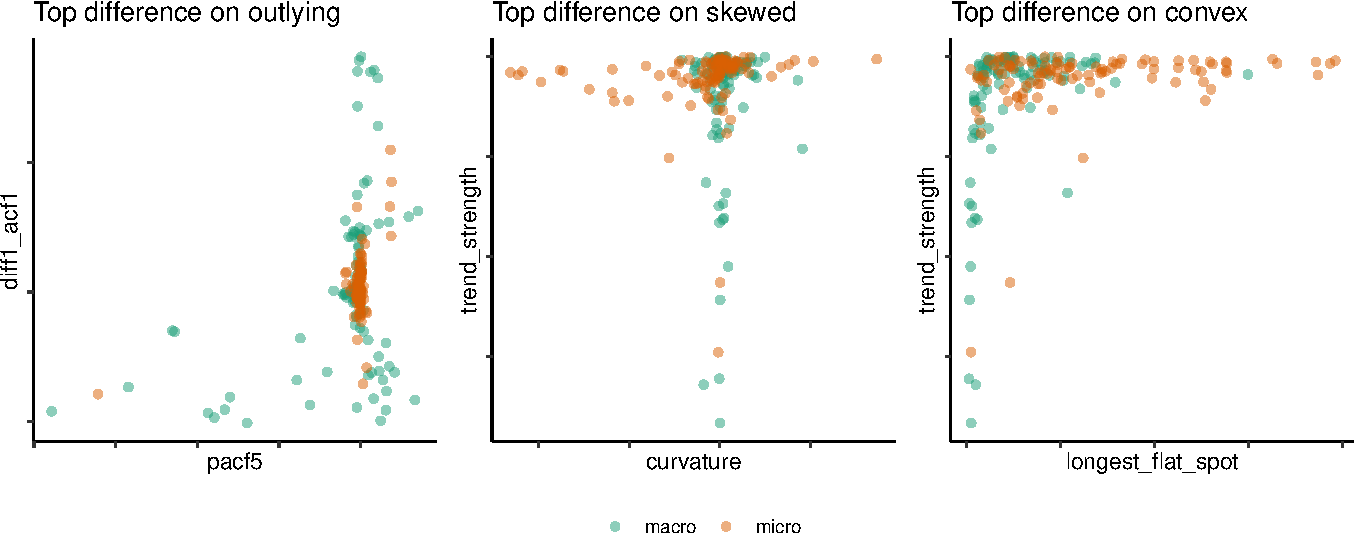
\includegraphics[width=1\linewidth]{mason-lee-laa-cook_files/figure-latex/timeseries-1} \caption[Interesting differences between two groups of time series detected by scagnostics]{Interesting differences between two groups of time series detected by scagnostics. The time series are described by time series features, in order to handle different length series. Scagnostics are computed on these features separately for each set to explore for shape differences.}(\#fig:timeseries)
\end{figure}
\end{Schunk}

\begin{Schunk}
\begin{figure}
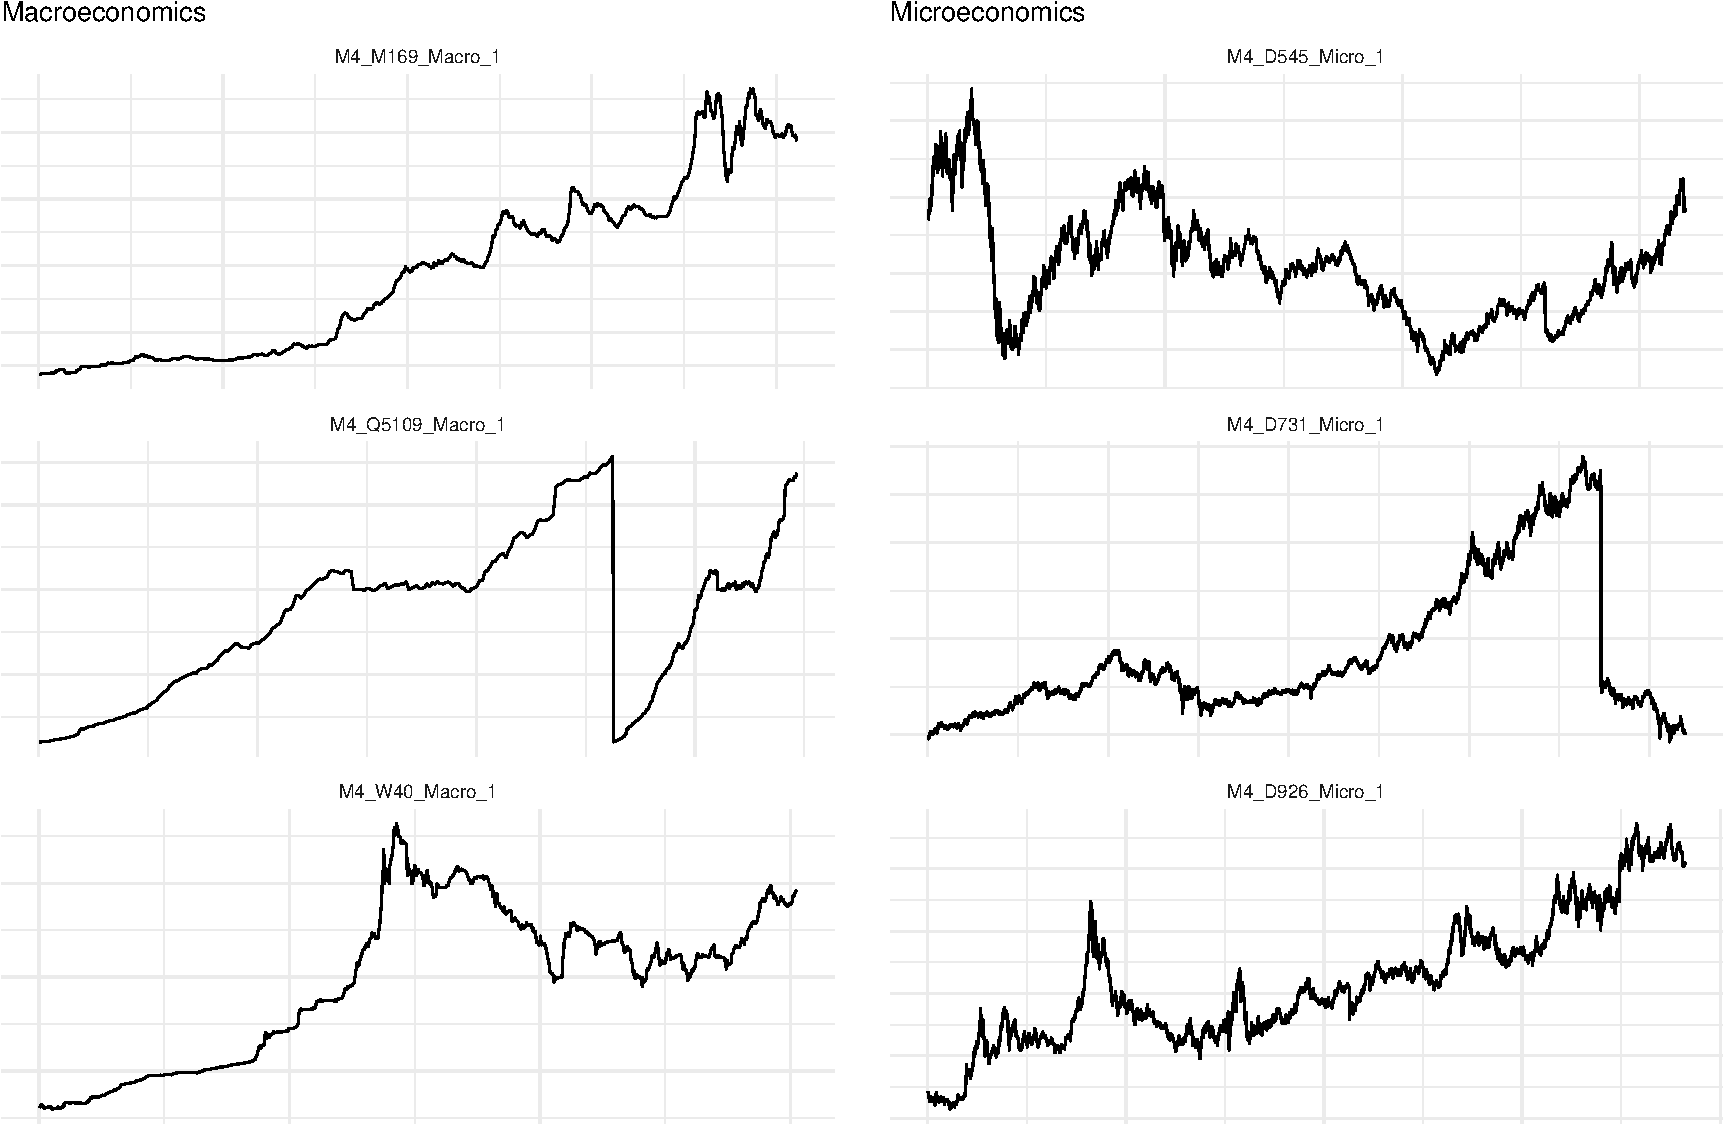
\includegraphics[width=1\linewidth]{mason-lee-laa-cook_files/figure-latex/tsplots-1} \caption[Selection of series from the two groups, macroeconomics and microeconomics]{Selection of series from the two groups, macroeconomics and microeconomics. The difference is in the jagginess of the two series.}(\#fig:tsplots)
\end{figure}
\end{Schunk}

\hypertarget{black-hole-mergers}{%
\subsection{Black hole mergers}\label{black-hole-mergers}}

We now use scagnostics to study a simulated dataset that contains
posterior samples describing a gravitational waves signal from a black
hole merger. The data contains 13 variables that describe the event in
terms of: its position in the sky (three variables: ra, dec, distance),
the time of the event (time), the black hole properties (masses m1 and
m2; spin related properties alpha, theta\_jn, chi\_tot, chi\_eff,
chi\_p), and additional nuisance parameters psi (polarisation angle) and
phi\_jl (orbital phase). In this example looking at the complete SPLOM
is still feasible, and could be used to identify several interesting
scatterplots and the corresponding combination of variables. Most
notably we can see non-linear and non-functional relations between pairs
of variables, and we expect that these should stand out on the
scagnostics measures as well.

The full data file contains 9998 posterior samples, without binning it
is too long to compute the scagnostics on such a large number of
observations. For our purpose a much smaller sample is sufficient, and
we randomly sample 200 observations before computing the scagnostics.

\begin{Schunk}
\begin{figure}
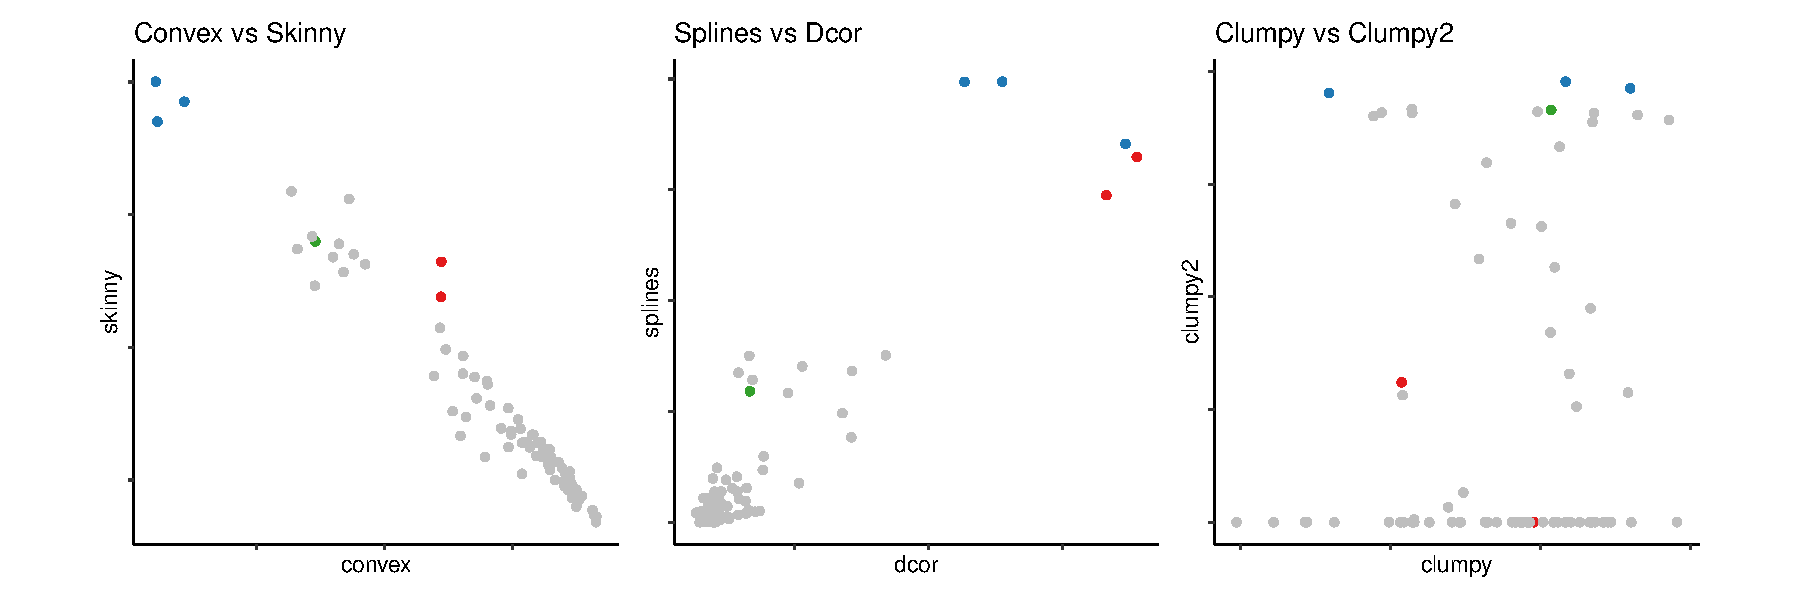
\includegraphics[width=1\linewidth]{mason-lee-laa-cook_files/figure-latex/bbh-scags-static-1} \caption[Pairs of scagnostics computed for the black hole mergers data]{Pairs of scagnostics computed for the black hole mergers data. XXX}(\#fig:bbh-scags-static)
\end{figure}
\end{Schunk}

Figure @ref(fig:bbh-scags-static) shows scatterplots of the computed
scagnostics measures, where several combinations stand out. On the left
plot we see three points with very low values of the convex measure and
high values of skinny. These are all possible combinations containing
the variables time, ra and dec, and the corresponding scatterplots are
shown in the upper row of Figure @ref(fig:blackholes). Because of how a
single experiment observes the sky, there is an interesting pattern
between these variables, with posterior samples being drawn along a
non-linear band in this three-dimensional space.

These variables also stand out in the middle plot of Figure
@ref(fig:bbh-scags-static), where it is interesting to note that the
cominations with non-linear but functional relation (time vs ra and dec
vs ra) have somewhat higher values in the splines measure compared to
dcor. On the other hand dec vs time does not exhibit a functional
relation, and consequently gets a higher dcor score compared to splines
(with both measures still taking large values). This also happens for
two other combinations: m1 vs m2 and chi\_p vs chi\_tot, which are shown
in the bottom row (left and middle) of Figure @ref(fig:blackholes). We
see that both these combinations show noisy linear relations.

Another interesting aspect with this dataset is that there are several
combinations that lead to visible separations between groups of points.
It is thus an ideal testcase for our new implementation of clumpy2. The
right plot in Figure @ref(fig:bbh-scags-static) shows clumpy vs clumpy2,
and reveals large differences between the two measures. In particular
there are many combinations without visible clustering, that still score
high on clumpy, but where clumpy2 is zero. On the other hand we can see
that there are several combinations that do lead to visible separation
between groups that stand out in terms of clumpy2, but not the original
clumpy. One example is time vs alpha, shown in the bottom right plot of
Figure @ref(fig:blackholes).

\begin{Schunk}
\begin{figure}
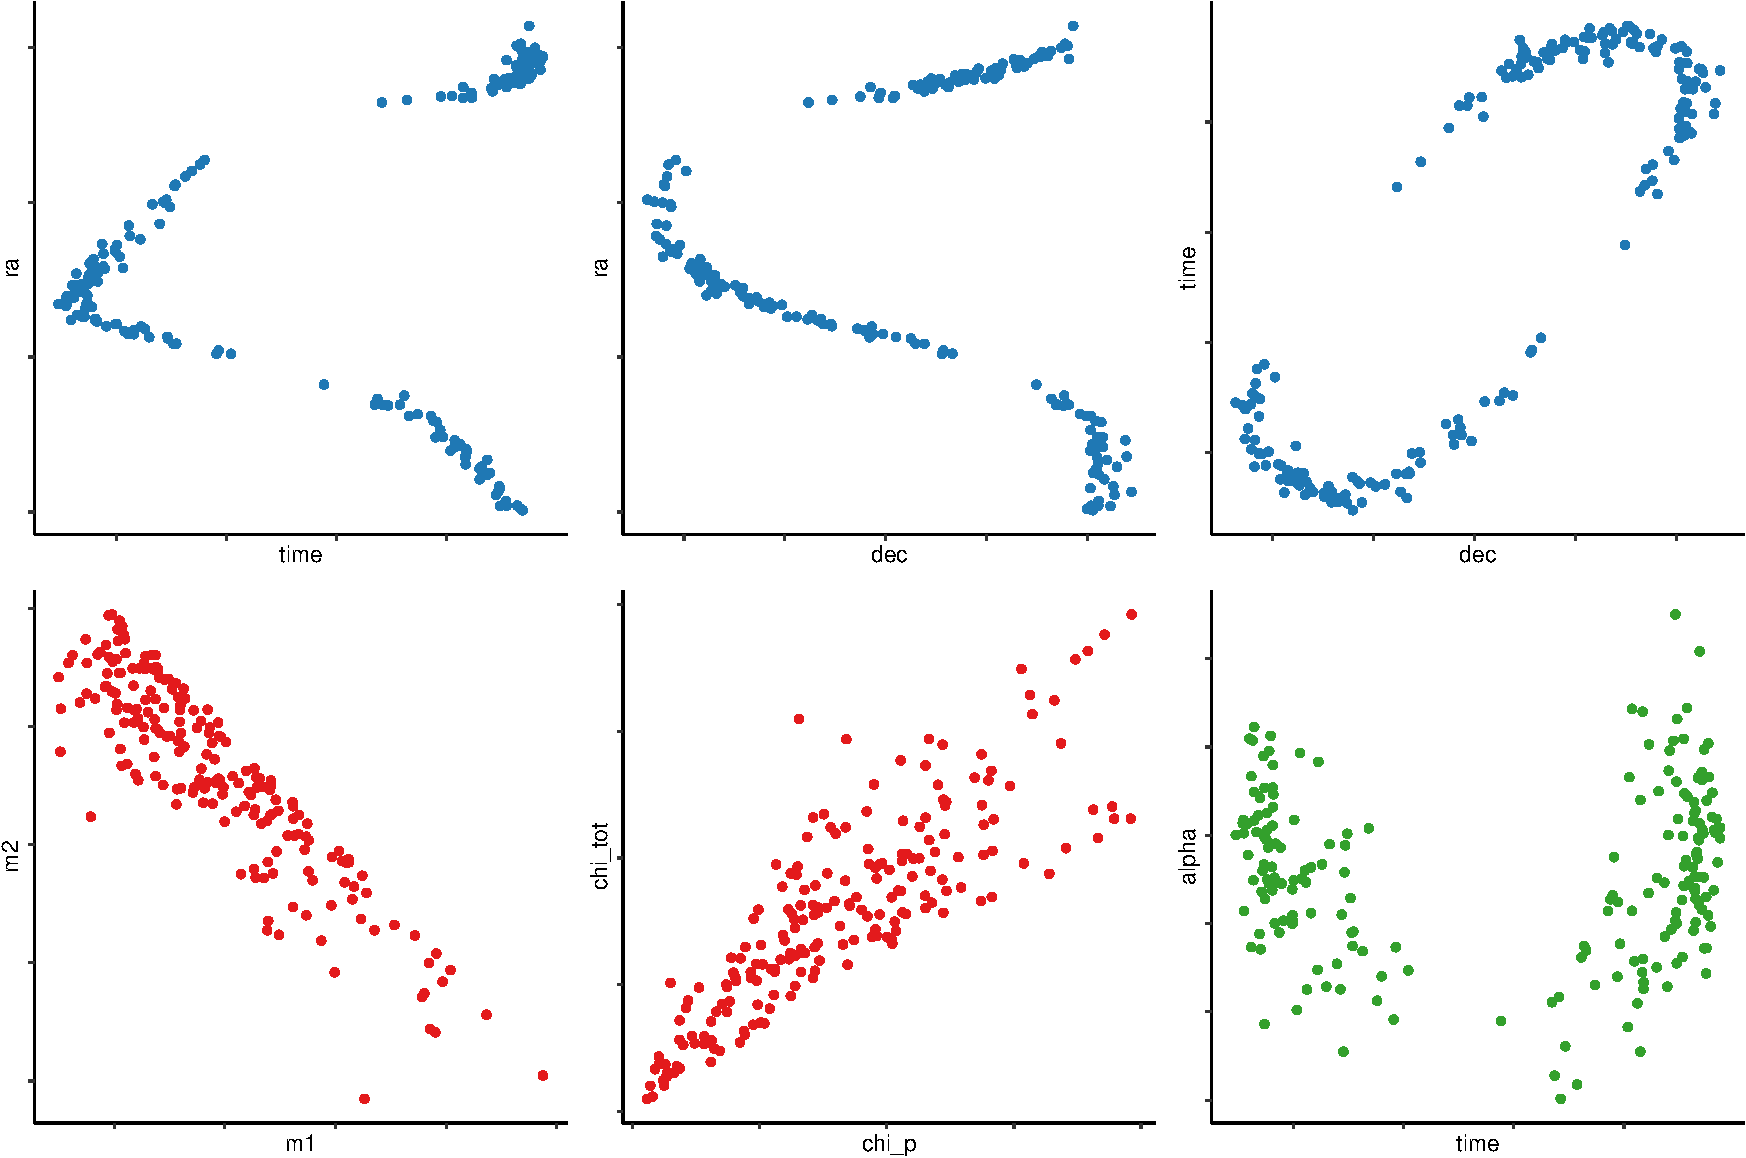
\includegraphics[width=1\linewidth]{mason-lee-laa-cook_files/figure-latex/blackholes-1} \caption[Features in the BBH data that stand out on several of the scagnostics measures (convey, skinny, splines and dcor), showing strong relations between variables including non-linear and non-functional dependencies]{Features in the BBH data that stand out on several of the scagnostics measures (convey, skinny, splines and dcor), showing strong relations between variables including non-linear and non-functional dependencies. The final example (time vs alpha) is expected to take high values in clumpy, but only stands out on the corrected clumpy2.}(\#fig:blackholes)
\end{figure}
\end{Schunk}

\hypertarget{afl-player-statistics}{%
\subsection{AFL player statistics}\label{afl-player-statistics}}

The Australian Football League Women's (AFLW) is the national
semi-profesisonal Australia Rules football league for female players.
Here we will analyse data sourced from the official AFL website with
information on the 2020 season, in which the league had 14 teams and
1932 players. There are 68 variables, 38 of which are numeric. The
others are categorical, like the players names or match ids, which would
not be used in scagnostic calculations. These numeric variables are
recorded per player per game, and a description of each variable in this
data set can be found in the appendix. With 33 numeric variables, there
are 528 possible scatterplots to make. This is much more than we could
possibly plot ourselves, and so we can use the scagnostics to identify
which might be interesting to examine ourselves. The figure below
displays 5 scatter plots that were identified as having a particularly
high or low value on a scagnostic, or an unusual combination of two or
more scagnostics. In addition to these 5, there is a 6th plot that is
included to display what a middling value on almost all of the
scagnostics looks like. You may like to test your scagnostics knowledge
by guessing which plot is the middling value on all the scagnsotics.

\begin{Schunk}


\begin{center}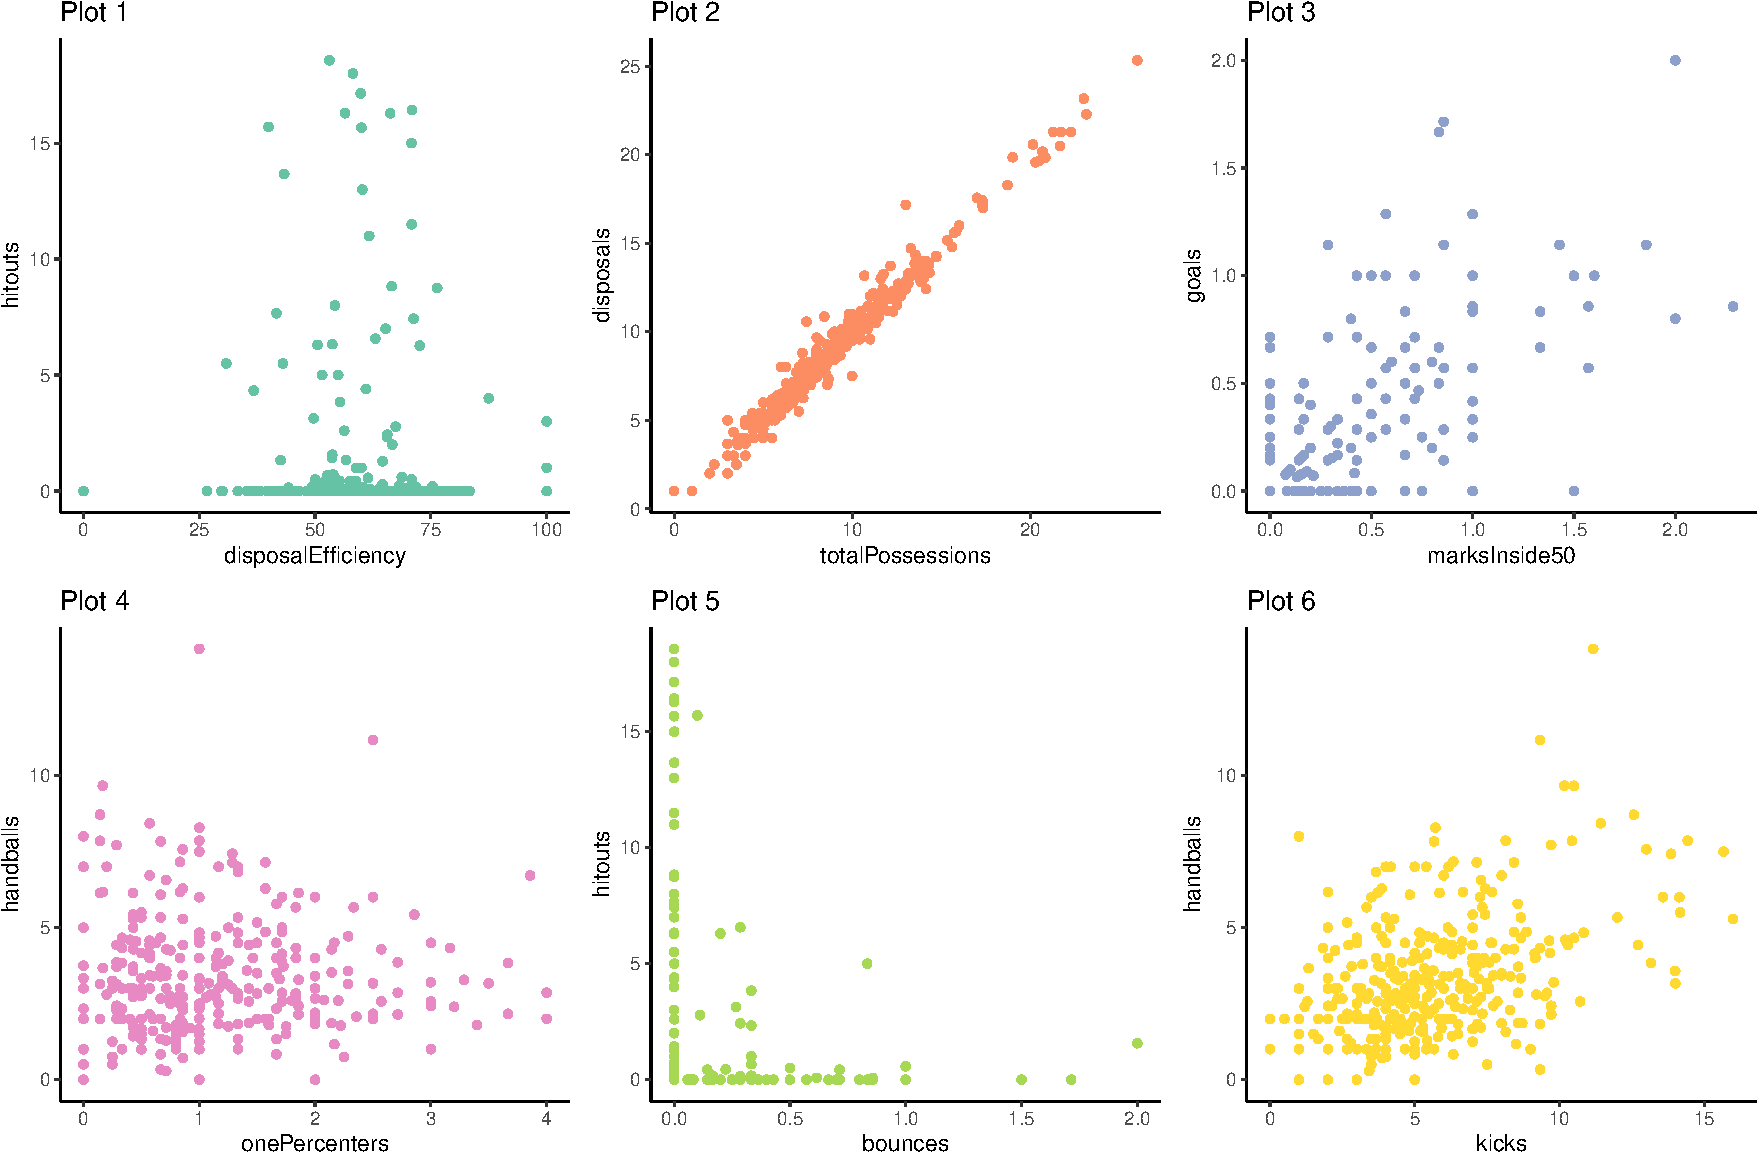
\includegraphics[width=0.8\linewidth]{mason-lee-laa-cook_files/figure-latex/AFLW-scatters-static-1} \end{center}

\end{Schunk}

Plots 1 to 5 are examples of unusual combinations of scagnostics, Plot 6
is an example of a scatter plot that was had moderate values across all
the scagnostics and was mostly picked at random. We can present Plot 6
alongside two other scatter plots that were selected arbitrarily (the
same way we would if we were going to try and do EDA ourselves) to give
an idea of what we would get if we arbitrarily selected variables to
plot.

\begin{Schunk}


\begin{center}\includegraphics[width=1\linewidth]{mason-lee-laa-cook_files/figure-latex/3 Random Plots-1} \end{center}

\end{Schunk}

We could plot scatter plots like this all day, but most of the scatter
plots in this data set look something like this, and when compared to
Plots 1 to 5 we can see that the extreme values on the scagnostic
measurements identify atypical scatter plots. While it is interesting to
know that scagnostics can pick out interesting scatter plots, we still
need to know how to use them. Typically the plots with strange
scagnostic combinations are identified using an interactive SPLOM, but
for the sake of space, we are only going to show the specific scatter
plots of the SPLOM that led to the selection of Plots 1, 2, and 5. Lets
start with Plot 1.

\hypertarget{plot-1}{%
\paragraph{Plot 1}\label{plot-1}}

We identified Plot 1 as interesting as it returned high values on both
Outlying and Skewed. This indicates that even after removing outliers,
the data was still disproportionately spread out, a trend we can see
very clearly in the identified scatter plot.

\begin{Schunk}


\begin{center}\includegraphics[width=0.7\linewidth]{mason-lee-laa-cook_files/figure-latex/plot1-static-1} \end{center}

\end{Schunk}

\hypertarget{plot-2}{%
\paragraph{Plot 2}\label{plot-2}}

Plot 2 scored very highly on all the association measures, which
indicates a strong relationship between the two variables. The three
association measures typically have strong correlation, and scatter
plots that stay within the large mass in the center have a linear
relation, scatter plots that deviate from this large correlation
typically have some strong non-linear relationship. Unfortunately that
does not appear here, and so none of these variable pairs have strong
non-linear relationships, rather our highest scagnostic on the
association measures indicates the linear relationship between total
posessions and disposals. Total possessions is the number of times the
player has the ball and disposals is the number of times the player gets
rid of the ball legally, so the high correlation makes sense, this is a
professional league so most of the players succeed in getting rid of the
ball legally.

\begin{Schunk}


\begin{center}\includegraphics[width=0.7\linewidth]{mason-lee-laa-cook_files/figure-latex/plot2-static-1} \end{center}

\end{Schunk}

\hypertarget{plot-5}{%
\paragraph{Plot 5}\label{plot-5}}

This plot is an excellent example in what new information we can learn
from a unique pairwise relationship. This scatter plot is separate from
the mass of pairwise relationships because it was high on striated\_2
and low on outlying, which tells us most of the points are at right
angles and a little spread out (but not enough for a high outlying
value). This plot tells us something interesting about the physicality
of the players. If a specific sports statistic is related to position,
we would see a relationship have a lower triangular structure similar to
that of Plot 4, however this plot does not have a lower triangular
structure, is has an L-shape. This means these statistics are not about
position, but rather the physical abilities of the players. Hitouts
measure the number of times the player punches the ball after the
referee throws it back into play, bounces have to be done while running,
and are typically done by fast players. The l-shape tells us that
players who do one very rarely perform the other. The moderate spread
along both of the statistics tells us these are both somewhat
specialised skills, and the players who specialise in one do not
specialise in the other, i.e.~in AFL the tallest player in the team is
rarely the fastest.

\begin{Schunk}


\begin{center}\includegraphics[width=0.7\linewidth]{mason-lee-laa-cook_files/figure-latex/plot5-static-1} \end{center}

\end{Schunk}

\hypertarget{splines-work}{%
\subsubsection{Splines Work}\label{splines-work}}

\begin{Schunk}


|Var1                       |Var2                          | splines|
|:--------------------------|:-----------------------------|-------:|
|totalPossessions           |disposals                     |    0.94|
|clearances.totalClearances |clearances.stoppageClearances |    0.88|
|goalAccuracy               |goals                         |    0.83|
|metresGained               |kicks                         |    0.77|
|dreamTeamPoints            |disposals                     |    0.74|
|disposals                  |kicks                         |    0.72|
|dreamTeamPoints            |totalPossessions              |    0.72|
|totalPossessions           |uncontestedPossessions        |    0.68|
|dreamTeamPoints            |kicks                         |    0.67|
|uncontestedPossessions     |disposals                     |    0.66|

\end{Schunk}

\begin{Schunk}
\begin{figure}
\includegraphics[width=1\linewidth]{mason-lee-laa-cook_files/figure-latex/aflwstatic-1} \caption[Scatterplots with high values on the splines scagnostic]{Scatterplots with high values on the splines scagnostic.}(\#fig:aflwstatic)
\end{figure}
\end{Schunk}

Figure @ref(fig:aflwstatic) shows three scatterplots that score highly
on the splines scagnostic. Each of these shows a relatively strong
monotonic relationship between the two variables. In the interactive
version of the plot, mouse over reveals some high-performing players,
e.g.~Anne Hatchard has a lot of possessions, disposals and kicks, and
Kaitlyn Ashmore kicked 4 goals in a match with 100\% accuracy.

NOTE: Each player is represented multiple times here, I think. The stats
are per game. Maybe it is better to aggregate for each player and re-do
the statistics?

\hypertarget{world-bank-development-indicators}{%
\subsection{World Bank Development
Indicators}\label{world-bank-development-indicators}}

The World Bank delivers a lot of development indicators \citep{WBI}, for
many countries and multiple years. The sheer volume of indicators, in
addition to substantial missing values, makes a barrier to analysis.
This is a good example to where scagnostics can be used to identify
pairs of indicators with interesting relationships.

Here we have downloaded indicators from 2018 for a number of countries.
First, the data needs some pre-processing, to remove variables which
have mostly missing values, and countries which have mostly missing
values. The scagnostics will be calculated on the pairwise complete
data, so it is ok to leave a few sporadic missings. At the end of the
pre-processing, there are 20 indicators for 79 countries.

\begin{Schunk}
\begin{figure}
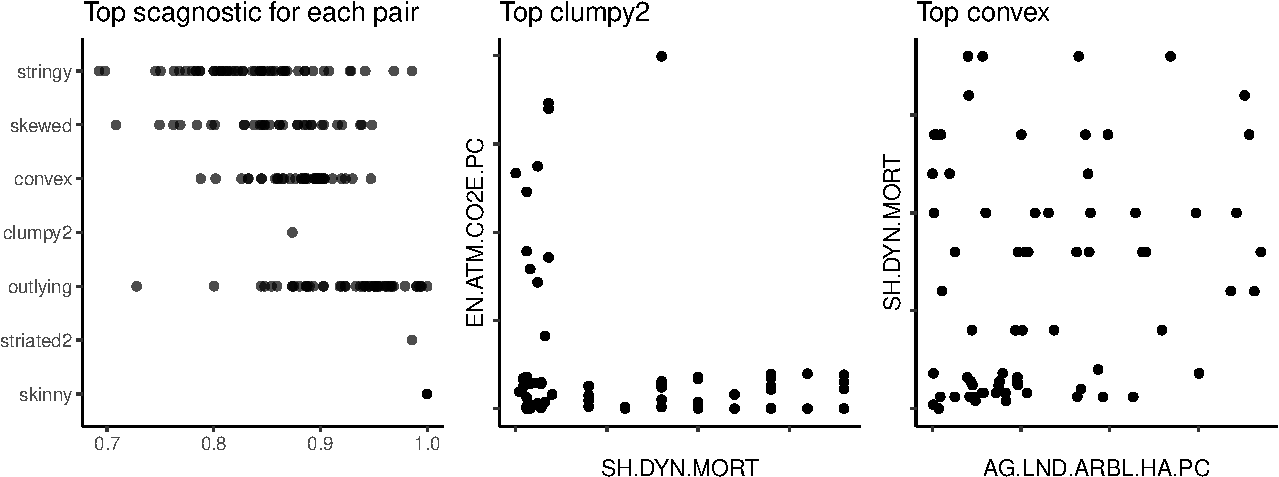
\includegraphics[width=1\linewidth]{mason-lee-laa-cook_files/figure-latex/wbistatic-1} \caption[Most of the pairs of indicators exhibit outliersor are stringy]{Most of the pairs of indicators exhibit outliersor are stringy. There is one pair that has clumpy as the highest value. There are numerous pairs that have a highest value on convex.}(\#fig:wbistatic)
\end{figure}
\end{Schunk}

\hypertarget{summary}{%
\subsection{Summary}\label{summary}}

\hypertarget{appendix}{%
\section{Appendix}\label{appendix}}

\hypertarget{aflw-data-variable-descriptions}{%
\subsection{AFLW Data Variable
Descriptions}\label{aflw-data-variable-descriptions}}

\begin{itemize}
\tightlist
\item
  \emph{timeOnGroundPercentage}: percentage of the game the player was
  on the field.\\
\item
  \emph{goals}: the 6 points a team gets when the kick the ball between
  the two big posts.\\
\item
  \emph{behinds}: the 1 point a team gets when they kick the ball
  between the big post and small post.\\
\item
  \emph{kicks}: number of kicks done by the player in this game.\\
\item
  \emph{handballs}: number of handballs does by the player in the
  game.\\
\item
  \emph{disposals}: the number kicks and handballs a player has.\\
\item
  \emph{marks}: total number of marks in the game (the ball travels more
  than 15m and the player catches it without another player touching it
  or it hitting the ground).\\
\item
  \emph{bounces}: the number of times a player bounced the ball in a
  game. A player must bounce the ball if they travel more than 15m and
  they can only bounce the ball once.\\
\item
  \emph{tackles}: Number of tackles performed by the player.\\
\item
  \emph{contestedPossessions}: the number of disposals a player has
  under pressure, i.e if a player is getting tackled and the get a
  handball or kick out of the scuffle.\\
\item
  \emph{uncontestedPossessions}: the number of disposals a player has
  under no pressure where they have space and time to get rid of the
  ball.\\
\item
  \emph{totalPossessions}: The total number of time the player has the
  ball.
\item
  \emph{inside50s}: the number of times the player has the ball within
  the 50m arc around the oponents goals.\\
\item
  \emph{marksInside50}: the number of marks a player gets within the 50m
  arc around the oponents goals.\\
\item
  \emph{contestedMarks}: the number of marks a player has under
  pressure.
\item
  \emph{hitouts}: this is how many times a player or team taps or
  punching the ball from a stoppage.
\item
  \emph{onePercenters}: all the things a player can do without
  registering a disposal. Eg. Spoils (punching the ball to stop someone
  from marking it), Shepparding (blocking for a teammate), smothering.\\
  \emph{disposalEfficiency}: a measure of how well a player disposes of
  the ball. E.g. if a player kicks or handballs to the opposition a lot,
  they will have a low disposal efficiency percentage.\\
\item
  \emph{clangers}: this is how many times a player or team dispose of
  the ball and it results in a turnover to the other team.\\
\item
  \emph{freesFor}: this player was awarded a free kick.\\
\item
  \emph{freesAgainst}: this player caused a free kick to be awarded to
  the other team.\\
\item
  \emph{dreamTeamPoints}: this is fantasy football scoring points.\\
\item
  \emph{rebound50s}: how many times the player exits the ball out of
  their defence 50m arc.\\
\item
  \emph{goalAssists}: number of times the player gave the pass
  immediately before the player that scored a goal.
\item
  \emph{goalAccuracy}: percentage ratio of the number of goals kicked to
  the number of goal attempts.\\
\item
  \emph{turnovers}: this players disposal caused a turnover (the ball
  touches the ground and the other team get it).\\
\item
  \emph{intercepts}: number of times this player intercepts the disposal
  of the other team.
\item
  \emph{tacklesInside50}: number of tackles performed by this player
  within their defence 50m arc.\\
\item
  \emph{shotsAtGoal}: number of total shots at goal for this player (sum
  of goals, behinds and misses)
\item
  \emph{scoreInvolvements}: number of times the player was involved in a
  passage of play leading up to a goal.
\item
  \emph{metresGained}: how far a player has been able to advance the
  ball without turning it over.\\
\item
  \emph{clearances.centreClearances}: this is the clearance from the
  centre bounce after a goal or at the start of a quarter
\item
  \emph{clearances.stoppageClearances}: all the clearance from stoppages
  around the ground
\item
  \emph{clearances.totalClearances}: how many time a player or team
  clears the ball from a stoppage or from the centre
\end{itemize}

\begin{verbatim}
\end{verbatim}

\bibliography{mason-lee-laa-cook.bib}

\address{%
Harriet Mason\\
Monash University\\%
Department of Econometrics and Business Statistics\\ Melbourne,
Australia\\
%
\url{https://www.britannica.com/animal/quokka}\\%
\textit{ORCiD: \href{https://orcid.org/0000-1721-1511-1101}{0000-1721-1511-1101}}\\%
\href{mailto:hmas0003@student.monash.edu}{\nolinkurl{hmas0003@student.monash.edu}}%
}

\address{%
Stuart Lee\\
Genentech\\%
\\
%
\url{https://stuartlee.org}\\%
\textit{ORCiD: \href{https://orcid.org/0000-0003-1179-8436}{0000-0003-1179-8436}}\\%
\href{mailto:stuart.andrew.lee@gmail.com}{\nolinkurl{stuart.andrew.lee@gmail.com}}%
}

\address{%
Ursula Laa\\
University of Natural Resources and Life Sciences\\%
Institute of Statistics\\ Vienna, Austria\\
%
\url{https://uschilaa.github.io}\\%
\textit{ORCiD: \href{https://orcid.org/0000-0002-0249-6439}{0000-0002-0249-6439}}\\%
\href{mailto:ursula.laa@boku.ac.at}{\nolinkurl{ursula.laa@boku.ac.at}}%
}

\address{%
Dianne Cook\\
Monash University\\%
Department of Econometrics and Business Statistics\\ Melbourne,
Australia\\
%
\url{https://dicook.org}\\%
\textit{ORCiD: \href{https://orcid.org/000-0002-3813-7155}{000-0002-3813-7155}}\\%
\href{mailto:dicook@monash.edu}{\nolinkurl{dicook@monash.edu}}%
}
